% =====================================================================
%  AyurMind - Codebase Documentation
%  Build:  pdflatex ayurmind_docs.tex  (run twice for the ToC)
% =====================================================================
\documentclass[11pt,a4paper]{report}

% ---------- encoding & fonts ----------
\usepackage[T1]{fontenc}
\usepackage[utf8]{inputenc}
\usepackage{lmodern}
\usepackage{microtype}

% ---------- layout ----------
\usepackage[a4paper,margin=2.4cm,headheight=22pt]{geometry}
\usepackage{fancyhdr}
\usepackage{titlesec}
\usepackage{parskip}
\usepackage{enumitem}
\setlist{itemsep=2pt,parsep=0pt,topsep=4pt}

% ---------- tables ----------
\usepackage{booktabs}
\usepackage{longtable}
\usepackage{array}
\usepackage{tabularx}
\usepackage{multirow}

% ---------- graphics ----------
\usepackage{xcolor}
\usepackage{graphicx}
\usepackage{tikz}
\usetikzlibrary{positioning,arrows.meta,shapes.geometric,calc,fit,backgrounds,decorations.pathreplacing,patterns}
\usepackage{pgfplots}
\pgfplotsset{compat=1.17}
\usepackage{float}
\usepackage{caption}
\captionsetup{font=small,labelfont=bf}

% ---------- code ----------
\usepackage{listings}

% ---------- boxes ----------
\usepackage[most]{tcolorbox}

% ---------- links (load late) ----------
\usepackage[colorlinks=true,linkcolor=deepgreen,citecolor=deepgreen,
            urlcolor=linkblue,pdftitle={AyurMind Codebase Documentation},
            pdfauthor={AyurMind}]{hyperref}

% =====================================================================
%  Palette
% =====================================================================
\definecolor{deepgreen}{HTML}{2E6B4F}
\definecolor{midgreen}{HTML}{4A9370}
\definecolor{palegreen}{HTML}{E8F2EC}
\definecolor{clay}{HTML}{B5651D}
\definecolor{paleclay}{HTML}{FBEEE2}
\definecolor{ink}{HTML}{22282B}
\definecolor{slate}{HTML}{5A6670}
\definecolor{linkblue}{HTML}{1F5C8B}
\definecolor{palegrey}{HTML}{F4F5F6}
\definecolor{rulegrey}{HTML}{D6DADC}
\definecolor{plum}{HTML}{6B3F84}
\definecolor{paleplum}{HTML}{F1EAF6}
\definecolor{amber}{HTML}{B08800}
\definecolor{paleamber}{HTML}{FDF6DC}
\definecolor{brick}{HTML}{A03A2E}
\definecolor{palebrick}{HTML}{FAE9E7}

% =====================================================================
%  Headers / footers
% =====================================================================
\pagestyle{fancy}
\fancyhf{}
\renewcommand{\headrulewidth}{0.4pt}
\renewcommand{\headrule}{\hbox to\headwidth{\color{rulegrey}\leaders\hrule height \headrulewidth\hfill}}
\fancyhead[L]{\small\color{slate}\nouppercase{\leftmark}}
\fancyhead[R]{\small\color{slate}AyurMind}
\fancyfoot[C]{\small\color{slate}\thepage}
\fancypagestyle{plain}{\fancyhf{}\fancyfoot[C]{\small\color{slate}\thepage}\renewcommand{\headrulewidth}{0pt}}

% =====================================================================
%  Section styling
% =====================================================================
\titleformat{\chapter}[display]
  {\normalfont\huge\bfseries\color{deepgreen}}
  {\normalsize\color{clay}\MakeUppercase{Chapter \thechapter}}
  {6pt}{\Huge}
\titlespacing*{\chapter}{0pt}{-20pt}{26pt}

\titleformat{\section}
  {\normalfont\Large\bfseries\color{deepgreen}}{\thesection}{0.7em}{}
\titleformat{\subsection}
  {\normalfont\large\bfseries\color{ink}}{\thesubsection}{0.7em}{}
\titleformat{\subsubsection}
  {\normalfont\normalsize\bfseries\color{slate}}{\thesubsubsection}{0.7em}{}

% =====================================================================
%  Code listing styles
% =====================================================================
\lstdefinestyle{py}{
  language=Python,
  basicstyle=\ttfamily\scriptsize,
  keywordstyle=\color{plum}\bfseries,
  commentstyle=\color{midgreen}\itshape,
  stringstyle=\color{clay},
  numbers=left,
  numberstyle=\ttfamily\tiny\color{slate},
  numbersep=6pt,
  showstringspaces=false,
  breaklines=true,
  breakatwhitespace=false,
  frame=leftline,
  framerule=2pt,
  rulecolor=\color{midgreen},
  framexleftmargin=24pt,
  xleftmargin=30pt,
  backgroundcolor=\color{palegrey},
  tabsize=4,
  captionpos=b,
  columns=fullflexible,
  keepspaces=true,
  literate={-}{-}1 {~}{{$\sim$}}1,
}

\lstdefinestyle{shell}{
  basicstyle=\ttfamily\scriptsize\color{ink},
  numbers=none,
  frame=leftline,
  framerule=2pt,
  rulecolor=\color{clay},
  framexleftmargin=6pt,
  xleftmargin=14pt,
  backgroundcolor=\color{paleclay},
  breaklines=true,
  showstringspaces=false,
  columns=fullflexible,
  literate={-}{-}1,
}

\lstdefinestyle{plain}{
  basicstyle=\ttfamily\scriptsize\color{ink},
  numbers=none,
  frame=leftline,
  framerule=2pt,
  rulecolor=\color{rulegrey},
  framexleftmargin=6pt,
  xleftmargin=14pt,
  backgroundcolor=\color{palegrey},
  breaklines=true,
  showstringspaces=false,
  columns=fullflexible,
  literate={-}{-}1,
}

\lstdefinestyle{json}{
  basicstyle=\ttfamily\scriptsize,
  stringstyle=\color{clay},
  numbers=none,
  frame=leftline,
  framerule=2pt,
  rulecolor=\color{plum},
  framexleftmargin=6pt,
  xleftmargin=14pt,
  backgroundcolor=\color{paleplum},
  breaklines=true,
  showstringspaces=false,
  columns=fullflexible,
  literate={-}{-}1,
}

\newcommand{\code}[1]{\texttt{\small #1}}
\newcommand{\fpath}[1]{\texttt{\small\color{deepgreen}#1}}

% let long monospace identifiers break rather than run into the margin
\setlength{\emergencystretch}{3em}
\hyphenpenalty=1000
\sloppy

% =====================================================================
%  Callout boxes
% =====================================================================
\tcbset{calloutbase/.style={
  enhanced, breakable, boxrule=0pt, leftrule=3pt, arc=1pt,
  left=8pt, right=8pt, top=6pt, bottom=6pt,
  fonttitle=\bfseries\small, coltitle=white, titlerule=0pt,
  attach boxed title to top left={xshift=3pt, yshift=-1mm},
  boxed title style={boxrule=0pt, arc=1pt, left=5pt, right=5pt,
                     top=2pt, bottom=2pt}}}

\newtcolorbox{note}[1][]{calloutbase, colback=palegreen, colframe=midgreen,
  colbacktitle=midgreen, #1}

\newtcolorbox{warn}[1][]{calloutbase, colback=paleamber, colframe=amber,
  colbacktitle=amber, #1}

\newtcolorbox{bug}[1][]{calloutbase, colback=palebrick, colframe=brick,
  colbacktitle=brick, #1}

% =====================================================================
%  TikZ node styles
% =====================================================================
\tikzset{
  blk/.style={rectangle, rounded corners=3pt, draw=#1, fill=#1!8,
              line width=0.9pt, align=center, inner sep=6pt,
              font=\footnotesize, minimum height=9mm},
  lyr/.style={rectangle, rounded corners=5pt, draw=#1!50, fill=#1!4,
              line width=0.7pt, dashed, inner sep=9pt},
  db/.style={cylinder, shape border rotate=90, aspect=0.28, draw=#1,
             fill=#1!8, line width=0.9pt, align=center, font=\footnotesize,
             inner sep=5pt, minimum height=11mm},
  dia/.style={diamond, aspect=2.2, draw=#1, fill=#1!8, line width=0.9pt,
              align=center, font=\scriptsize, inner sep=2pt},
  ar/.style={-{Stealth[length=2.4mm,width=1.8mm]}, line width=0.8pt, draw=slate},
  arb/.style={-{Stealth[length=2.4mm,width=1.8mm]}, line width=1.1pt, draw=#1},
  lbl/.style={font=\scriptsize\itshape, color=slate, fill=white, inner sep=1.5pt},
  lifeline/.style={draw=rulegrey, line width=0.7pt, dash pattern=on 2pt off 2pt},
}

% =====================================================================
\begin{document}

% ---------------------------------------------------------------
%  TITLE PAGE
% ---------------------------------------------------------------
\begin{titlepage}
\centering
\vspace*{1.2cm}


\begin{tikzpicture}
  \fill[deepgreen] (0,0) rectangle (16,0.16);
\end{tikzpicture}

\vspace{1.4cm}

{\fontsize{46}{50}\selectfont\bfseries\color{deepgreen} AyurMind\par}

\vspace{0.5cm}
{\LARGE\color{ink} Codebase Documentation\par}

\vspace{0.35cm}
{\large\color{slate} A multi-agent retrieval system over the Charaka Samhita\par}

\vspace{1.8cm}

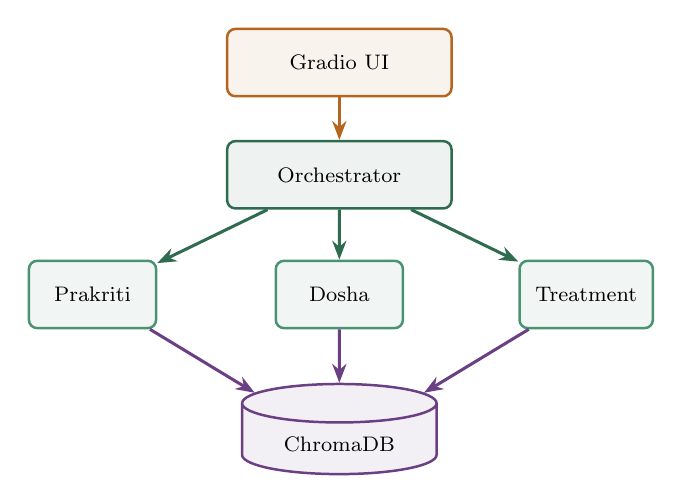
\begin{tikzpicture}[scale=0.95, transform shape]
  \node[blk=clay,   minimum width=30mm] (ui)   at (0,0)    {Gradio UI};
  \node[blk=deepgreen, minimum width=30mm] (or) at (0,-1.5) {Orchestrator};
  \node[blk=midgreen, minimum width=17mm] (a1) at (-3.3,-3.1) {Prakriti};
  \node[blk=midgreen, minimum width=17mm] (a2) at (0,-3.1)    {Dosha};
  \node[blk=midgreen, minimum width=17mm] (a3) at (3.3,-3.1)  {Treatment};
  \node[db=plum, minimum width=26mm] (db) at (0,-5.1) {ChromaDB};

  \draw[arb=clay]  (ui) -- (or);
  \draw[arb=deepgreen] (or) -- (a1);
  \draw[arb=deepgreen] (or) -- (a2);
  \draw[arb=deepgreen] (or) -- (a3);
  \draw[arb=plum] (a1) -- (db);
  \draw[arb=plum] (a2) -- (db);
  \draw[arb=plum] (a3) -- (db);
\end{tikzpicture}

\vfill

{\large\color{ink}Repository: \code{AyurMind}\par}
\vspace{0.2cm}
{\color{slate} Documented from commit \code{9213703} on branch \code{main}\par}
\vspace{0.2cm}
{\color{slate} 26 July 2026\par}

\vspace{1.2cm}

\begin{tikzpicture}
  \fill[clay] (0,0) rectangle (16,0.16);
\end{tikzpicture}
\end{titlepage}

% ---------------------------------------------------------------
\pagenumbering{roman}
\setcounter{tocdepth}{2}
\tableofcontents
\cleardoublepage
\pagenumbering{arabic}

\chapter{What AyurMind Is}

AyurMind answers health questions in the vocabulary of classical Ayurveda, and it tries to answer them from a book rather than from memory. The book is the Charaka Samhita, scraped from \href{https://www.carakasamhitaonline.com}{carakasamhitaonline.com}, cut into roughly 800-token passages, embedded with a sentence-transformer model, and stored in a local ChromaDB collection called \code{ayurvedic\_texts}. When you ask a question, the system searches that collection, hands the matching passages to a language model along with a role-specific instruction, and assembles the answers into a consultation report.

The part that makes it more than a plain retrieval chatbot is the split into four roles. Three specialist agents each own one clinical task and each search a different slice of the corpus. A fourth agent, the orchestrator, decides which specialists to wake up, feeds each one's output into the next, and writes the final report. A question about diet alone touches one agent; a question describing symptoms, constitution, and a request for a remedy touches all three.

\section{The problem it targets}

Two things go wrong when a general-purpose language model is asked an Ayurvedic question. It invents plausible-sounding Sanskrit that has no textual basis, and it flattens the distinction between constitution (\emph{Prakriti}, what you were born with) and current imbalance (\emph{Vikriti}, what is wrong right now). A treatment that ignores that distinction can be actively wrong: a warming, oily regimen that settles Vata will aggravate a Pitta patient.

The design responds to both. Grounding is handled by retrieval --- every specialist prompt carries retrieved passages and the model is told to answer from them. The Prakriti/Vikriti distinction is handled structurally, by giving each concept its own agent, its own system prompt, and its own metadata filter over the corpus.

\section{Who the output is written for}

The system prompts are unusually specific about audience. All three specialists and the orchestrator are told they are addressing BAMS graduates and practitioners, and are instructed to use Sanskrit clinical terminology, cite the classical section a recommendation comes from, and drop conversational framing. From \fpath{src/agents/orchestrator.py}:

\begin{lstlisting}[style=plain]
- Precision over Personability: Prioritize clinical accuracy and detailed
  explanations over conversational pleasantries. Avoid "friendly" or
  "approachable" language. Do not use phrasings like "Let me explain..."
\end{lstlisting}

That choice explains a lot of the code. It is why the synthesis prompt enforces a four-heading report structure, why the treatment agent must attach a supervision warning to any Panchakarma procedure, and why the evaluation harness asks BAMS practitioners rather than crowdworkers to score the outputs.

\section{The two paths through the system}

Every query hits \code{OrchestratorAgent.simple\_query()}, which does a keyword scan and then picks one of two routes.

\begin{figure}[H]
\centering
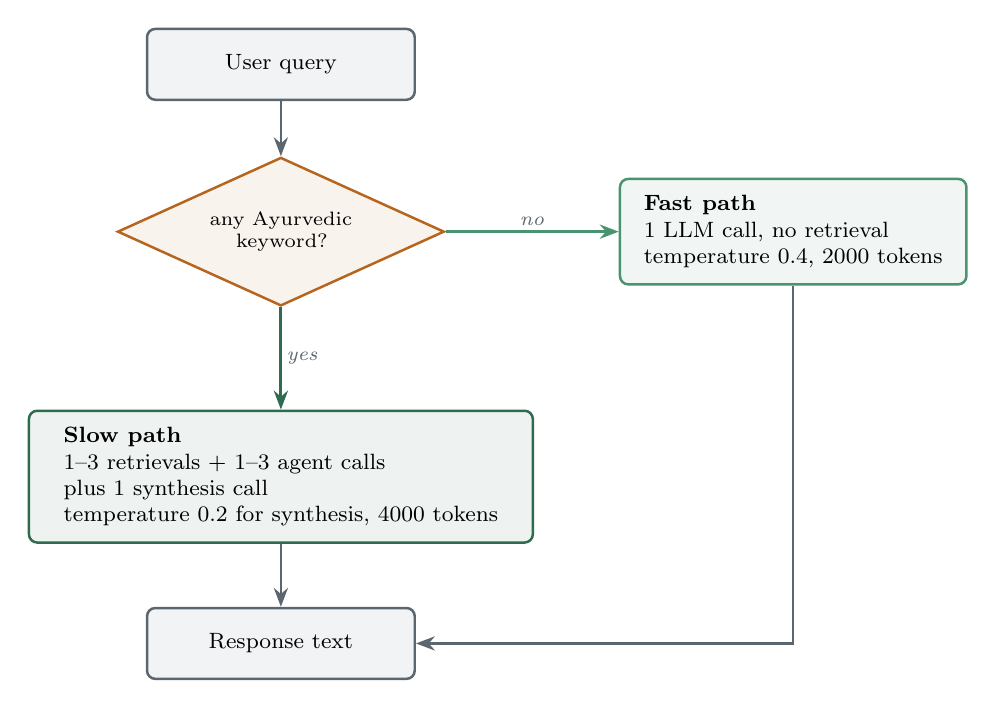
\begin{tikzpicture}[node distance=8mm]
  \node[blk=slate, minimum width=34mm] (q) {User query};
  \node[dia=clay, below=7mm of q, text width=26mm] (d) {any Ayurvedic\\keyword?};
  \node[blk=midgreen, right=22mm of d, minimum width=44mm, align=left] (fast)
       {\textbf{Fast path}\\1 LLM call, no retrieval\\temperature 0.4, 2000 tokens};
  \node[blk=deepgreen, below=13mm of d, minimum width=64mm, align=left] (slow)
       {\textbf{Slow path}\\1--3 retrievals + 1--3 agent calls\\plus 1 synthesis call\\temperature 0.2 for synthesis, 4000 tokens};
  \node[blk=slate, below=8mm of slow, minimum width=34mm] (out) {Response text};

  \draw[ar] (q) -- (d);
  \draw[arb=midgreen] (d) -- node[lbl,above]{no} (fast);
  \draw[arb=deepgreen] (d) -- node[lbl,right]{yes} (slow);
  \draw[ar] (slow) -- (out);
  \draw[ar] (fast.south) |- (out.east);
\end{tikzpicture}
\caption{Query routing. The keyword scan in \code{analyze\_query()} is the only gate; there is no model-based classifier.}
\end{figure}

The fast path exists for cost and latency. Asking ``what is Ayurveda?'' does not need three retrievals and four model calls, so it gets one call with a short, friendly system prompt. Everything else --- anything mentioning a dosha, a symptom, or a remedy --- takes the slow path.

\section{Technology in one table}

\begin{table}[H]
\centering
\small
\begin{tabularx}{\textwidth}{@{}l l X@{}}
\toprule
\textbf{Concern} & \textbf{Choice} & \textbf{Where it lives} \\
\midrule
Source text & Charaka Samhita, 8 sections & \fpath{src/scraper/charaka\_scraper.py} \\
Chunking & 800 tokens, 200 overlap, \code{cl100k\_base} & \fpath{src/scraper/data\_processor.py} \\
Embeddings & \code{all-mpnet-base-v2} (768-dim) & \fpath{src/rag/embeddings.py} \\
Vector store & ChromaDB, persistent on disk & \fpath{src/rag/vectorstore.py} \\
Default LLM & Gemini \code{gemini-1.5-flash} & \fpath{src/llm/google\_client.py} \\
Alternate LLMs & OpenAI, OpenRouter, Ollama & \fpath{src/llm/} \\
Agents & 3 specialists + 1 orchestrator & \fpath{src/agents/} \\
Interface & Gradio Blocks, port 7860 & \fpath{src/ui/gradio\_app.py} \\
Packaging & Dockerfile + compose, HF Spaces & \fpath{Dockerfile}, \fpath{app.py} \\
\bottomrule
\end{tabularx}
\caption{The stack as the code actually configures it.}
\end{table}

\begin{warn}[title={The README describes an older design}]
\fpath{README.md} names OpenRouter as the primary LLM provider, lists LangChain as the RAG framework, and shows Sushruta Samhita and Ashtanga Hridaya in the knowledge base. None of those are true of the current code: the default provider is Google Gemini, \code{langchain} is never imported despite being pinned in \fpath{requirements.txt}, and the scraper only covers Charaka. Chapter~\ref{ch:gaps} lists every divergence with the file that proves it. Read that chapter before trusting the README.
\end{warn}

\chapter{Repository Layout}

Seventy files are tracked in git. Roughly a third of them are source, a third are evaluation artefacts, and a third are documentation and diagrams. The tree below marks what each directory is responsible for.

\begin{lstlisting}[style=plain]
AyurMind/
|
|-- app.py                      entry point for Hugging Face Spaces
|-- Dockerfile                  python:3.10-slim image, CMD -> scripts/04_run_app.py
|-- docker-compose.yml          single service, port 7860, ./data mounted
|-- requirements.txt            pinned deps (some unused - see chapter 11)
|-- requirements_simplified.txt smaller variant, no langchain/jupyter
|
|-- scripts/                    the four-step pipeline, run in order
|   |-- 01_scrape_data.py       scrape + chunk           (15-30 min)
|   |-- 02_build_vectordb.py    embed + index            (5-10 min)
|   |-- 03_test_rag.py          three smoke queries      (1 min)
|   `-- 04_run_app.py           launch Gradio            (instant)
|
|-- src/
|   |-- scraper/
|   |   |-- charaka_scraper.py  CharakaScraper: fetch 8 sections -> data/raw/
|   |   `-- data_processor.py   AyurvedicTextProcessor: clean, chunk, tag
|   |-- rag/
|   |   |-- embeddings.py       EmbeddingGenerator: sentence-transformers
|   |   |-- vectorstore.py      AyurvedicVectorStore: ChromaDB wrapper
|   |   `-- retriever.py        RAGRetriever: embed query -> search -> chunks
|   |-- llm/
|   |   |-- google_client.py    GoogleClient    (default)
|   |   |-- openai_client.py    OpenAIClient    (USE_OPENAI=true)
|   |   |-- local_client.py     OllamaClient    (USE_LOCAL_LLM=true)
|   |   `-- openrouter_client.py OpenRouterClient (present, never imported)
|   |-- agents/
|   |   |-- base_agent.py       BaseAgent: retrieve -> prompt -> generate
|   |   |-- prakriti_agent.py   constitution, category filter "prakriti"
|   |   |-- dosha_agent.py      imbalance,    category filter "vikriti"
|   |   |-- treatment_agent.py  therapy,      category filter "treatment"
|   |   `-- orchestrator.py     routing, cascade, synthesis
|   `-- ui/
|       `-- gradio_app.py       AyurMindApp: wiring + chat handler
|
|-- evaluation/
|   |-- dataset/evaluation_cases.csv   40 labelled scenarios
|   |-- results/*.jsonl                raw model outputs, 40 lines each
|   |-- run_evaluation.py              driver (currently vanilla only)
|   |-- run_evaluation_REAL.py         driver for the full multi-agent run
|   |-- calculate_metrics.py           automated metrics + review templates
|   |-- generate_expert_templates.py   BAMS-facing CSV templates
|   `-- evaluation_summary_report.md   generated results table
|
|-- images/                     rendered PNGs of the two mermaid diagrams
|-- *.mermaid, *.mmd            architecture and dataflow diagram sources
|-- diagrams.html               standalone mermaid viewer
|-- prompts.txt                 20 hand-written test questions by category
`-- research_proposal.js        70 KB docx generator for the conference paper
\end{lstlisting}

\section{Directories the code creates but git ignores}

\fpath{.gitignore} excludes \code{data/} entirely, so nothing under it is in the repository. Three directories appear at runtime:

\begin{table}[H]
\centering
\small
\begin{tabularx}{\textwidth}{@{}l l X@{}}
\toprule
\textbf{Path} & \textbf{Created by} & \textbf{Contents} \\
\midrule
\code{data/raw/} & \code{CharakaScraper} & One folder per section: \code{index.html}, \code{chapter\_NN.html}, matching \code{.txt} files, \code{metadata.json}. Plus \code{scraping\_summary.json} at the top. \\
\code{data/processed/} & \code{AyurvedicTextProcessor} & \code{all\_chunks.json} (every chunk with text and metadata) and \code{processing\_summary.json}. \\
\code{data/vectordb/} & \code{AyurvedicVectorStore} & ChromaDB's SQLite file and index segments. Around 100~MB once populated. \\
\bottomrule
\end{tabularx}
\caption{Runtime data directories. A fresh clone has none of these; step 1 and step 2 of the pipeline build them.}
\end{table}

\begin{note}[title={The vector database is the deployment artefact}]
Everything before \fpath{scripts/02\_build\_vectordb.py} is a one-off. Once \code{data/vectordb/} exists you can throw away \code{data/raw/} and \code{data/processed/} --- the application only ever reads the Chroma collection. This matters for Docker and Hugging Face Spaces, where you want to ship the built database rather than scrape on every cold start.
\end{note}

\section{Files the README promises that do not exist}

\fpath{README.md} prints a project tree that includes a \code{tests/} package with three test modules, a \code{config/} directory holding \code{config.yaml} and \code{prompts.yaml}, a \code{notebooks/} folder, plus \code{.env.example}, \code{LICENSE}, and \code{CONTRIBUTING.md}. None of these are tracked in git. Prompts live inline as Python strings inside each agent class; configuration is read from environment variables through \code{os.getenv} at the point of use; there is no test suite, so the \code{pytest tests/} instruction in the README fails immediately.

\section{Reading order for a newcomer}

If you are opening this repository for the first time, the shortest path to understanding it is bottom-up, following the direction data actually moves:

\begin{enumerate}[leftmargin=*]
  \item \fpath{src/scraper/data\_processor.py} --- see what a chunk looks like and what metadata it carries. Everything downstream depends on those four metadata keys.
  \item \fpath{src/rag/vectorstore.py} --- 53 lines, and it shows exactly how the metadata is turned into a Chroma \code{where} filter.
  \item \fpath{src/agents/base\_agent.py} --- 63 lines that define the entire agent contract.
  \item \fpath{src/agents/orchestrator.py} --- the only file with real control flow.
  \item \fpath{src/ui/gradio\_app.py} --- the wiring that connects the four above.
\end{enumerate}

The four LLM clients can be skimmed; they are near-identical adapters around different HTTP APIs.

\chapter{Getting It Running}

\section{What you need}

Python 3.9 or newer, around 8~GB of RAM, and roughly 5~GB of free disk. The RAM figure is driven by \code{all-mpnet-base-v2}, which loads into memory at startup and stays there; the disk figure is the scraped HTML plus the Chroma index. You also need one of: a Google AI API key, an OpenAI API key, or a local Ollama installation.

\section{Install}

\begin{lstlisting}[style=shell]
git clone https://github.com/charansaiponnada/AyurMind.git
cd AyurMind

python -m venv venv
venv\Scripts\activate          # Windows
source venv/bin/activate        # macOS / Linux

pip install -r requirements.txt
\end{lstlisting}

\fpath{requirements.txt} pins 25 packages including Jupyter, black, flake8, mypy and pytest. For a runtime-only install, \fpath{requirements\_simplified.txt} drops the development tooling and the unused LangChain packages.

\section{Configuration}

There is no config file and no \code{.env.example} in the repository. Create \code{.env} yourself in the project root; \code{python-dotenv} loads it from both \fpath{src/ui/gradio\_app.py} and \fpath{src/scraper/charaka\_scraper.py}. A minimal working file is three lines:

\begin{lstlisting}[style=shell]
GOOGLE_API_KEY=your_key_here
GOOGLE_MODEL=gemini-1.5-flash
GRADIO_PORT=7860
\end{lstlisting}

Every variable the code reads, with the default it falls back to:

\begin{table}[H]
\centering
\small
\begin{tabularx}{\textwidth}{@{}l l X@{}}
\toprule
\textbf{Variable} & \textbf{Default} & \textbf{Read by} \\
\midrule
\multicolumn{3}{@{}l}{\textit{Provider selection}}\\
\code{USE\_LOCAL\_LLM} & \code{false} & \code{AyurMindApp.\_\_init\_\_} --- tries Ollama first \\
\code{USE\_OPENAI} & \code{false} & \code{AyurMindApp.\_\_init\_\_} --- tries OpenAI second \\
\midrule
\multicolumn{3}{@{}l}{\textit{Google (the default provider)}}\\
\code{GOOGLE\_API\_KEY} & --- & \code{GoogleClient}; raises \code{ValueError} if absent \\
\code{GOOGLE\_MODEL} & \code{gemini-1.5-flash} & \code{GoogleClient} \\
\midrule
\multicolumn{3}{@{}l}{\textit{OpenAI}}\\
\code{OPENAI\_API\_KEY} & --- & \code{OpenAIClient} \\
\code{OPENAI\_MODEL} & \code{gpt-4o-mini} & \code{OpenAIClient} \\
\midrule
\multicolumn{3}{@{}l}{\textit{Ollama}}\\
\code{LOCAL\_MODEL} & \code{llama3.2:3b} & \code{OllamaClient} \\
\midrule
\multicolumn{3}{@{}l}{\textit{OpenRouter (client exists, app never selects it)}}\\
\code{OPENROUTER\_API\_KEY} & --- & \code{OpenRouterClient} \\
\code{DEFAULT\_MODEL} & \code{mistralai/mistral-7b-instruct:free} & \code{OpenRouterClient} \\
\midrule
\multicolumn{3}{@{}l}{\textit{Retrieval}}\\
\code{EMBEDDING\_MODEL} & \code{sentence-transformers/all-mpnet-base-v2} & \code{EmbeddingGenerator} \\
\code{VECTOR\_DB\_PATH} & \code{./data/vectordb} & \code{AyurvedicVectorStore} \\
\code{MAX\_CHUNKS\_PER\_QUERY} & \code{5} & \code{RAGRetriever} \\
\midrule
\multicolumn{3}{@{}l}{\textit{Agents}}\\
\code{ORCHESTRATOR\_TEMP} & \code{0.2} & \code{OrchestratorAgent}, synthesis only \\
\midrule
\multicolumn{3}{@{}l}{\textit{Scraper}}\\
\code{REQUEST\_DELAY} & \code{2} & seconds between HTTP requests \\
\code{MAX\_RETRIES} & \code{3} & attempts per page \\
\code{TIMEOUT} & \code{30} & seconds per request \\
\midrule
\multicolumn{3}{@{}l}{\textit{Interface}}\\
\code{GRADIO\_PORT} & \code{7860} & \code{AyurMindApp.launch} \\
\code{GRADIO\_SHARE} & \code{false} & \code{AyurMindApp.launch}; also flips bind address \\
\bottomrule
\end{tabularx}
\caption{Complete environment variable reference, gathered from every \code{os.getenv} call in the codebase.}
\end{table}

\begin{warn}[title={Agent temperatures are hard-coded}]
Only the orchestrator's synthesis temperature is configurable. The three specialists set theirs in their constructors --- 0.3 for Prakriti and Dosha, 0.4 for Treatment --- and the fast path uses a literal \code{0.4}. Changing those means editing the agent files.
\end{warn}

\section{The four-step pipeline}

The scripts are numbered because each one consumes what the previous one produced. Running them out of order fails loudly rather than silently.

\begin{figure}[H]
\centering
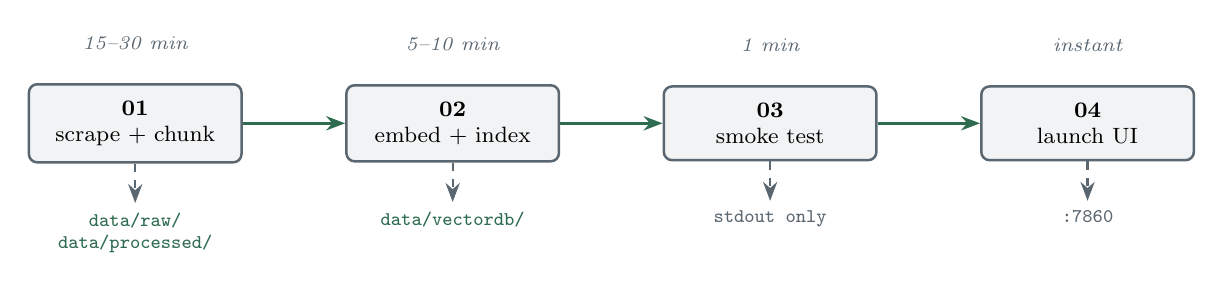
\begin{tikzpicture}[node distance=6mm]
  \node[blk=slate,  minimum width=27mm, align=center] (s1) {\textbf{01}\\scrape + chunk};
  \node[blk=slate,  minimum width=27mm, right=13mm of s1] (s2) {\textbf{02}\\embed + index};
  \node[blk=slate,  minimum width=27mm, right=13mm of s2] (s3) {\textbf{03}\\smoke test};
  \node[blk=slate,  minimum width=27mm, right=13mm of s3] (s4) {\textbf{04}\\launch UI};

  \node[font=\scriptsize\ttfamily, color=deepgreen, below=5mm of s1, align=center] (f1) {data/raw/\\data/processed/};
  \node[font=\scriptsize\ttfamily, color=deepgreen, below=5mm of s2, align=center] (f2) {data/vectordb/};
  \node[font=\scriptsize\ttfamily, color=slate, below=5mm of s3, align=center] (f3) {stdout only};
  \node[font=\scriptsize\ttfamily, color=slate, below=5mm of s4, align=center] (f4) {:7860};

  \node[font=\scriptsize\itshape, color=slate, above=3mm of s1] {15--30 min};
  \node[font=\scriptsize\itshape, color=slate, above=3mm of s2] {5--10 min};
  \node[font=\scriptsize\itshape, color=slate, above=3mm of s3] {1 min};
  \node[font=\scriptsize\itshape, color=slate, above=3mm of s4] {instant};

  \draw[arb=deepgreen] (s1) -- (s2);
  \draw[arb=deepgreen] (s2) -- (s3);
  \draw[arb=deepgreen] (s3) -- (s4);
  \draw[ar, dashed] (s1) -- (f1);
  \draw[ar, dashed] (s2) -- (f2);
  \draw[ar, dashed] (s3) -- (f3);
  \draw[ar, dashed] (s4) -- (f4);
\end{tikzpicture}
\caption{Pipeline stages with their runtimes and outputs. Only steps 1 and 2 write to disk.}
\end{figure}

\begin{lstlisting}[style=shell]
python scripts/01_scrape_data.py     # -> data/raw/ and data/processed/
python scripts/02_build_vectordb.py  # -> data/vectordb/
python scripts/03_test_rag.py        # prints three retrieval results
python scripts/04_run_app.py         # http://127.0.0.1:7860
\end{lstlisting}

Step 4 accepts a flag:

\begin{lstlisting}[style=shell]
python scripts/04_run_app.py --share
\end{lstlisting}

which sets Gradio's \code{share=True}, binds to \code{0.0.0.0} and produces a temporary public \code{gradio.live} URL. Setting \code{GRADIO\_SHARE=true} in \code{.env} does the same thing.

\subsection{What step 1 actually prints}

\fpath{scripts/01\_scrape\_data.py} runs two phases in one process --- \code{CharakaScraper.scrape\_all()} then \code{AyurvedicTextProcessor.process\_all()} --- and reports counts from both:

\begin{lstlisting}[style=py,firstnumber=36]
    print("SCRAPING COMPLETE!")
    print(f"Scraped {scraping_summary['total_sections']} sections")
    print(f"Total chapters: {scraping_summary['total_chapters']}")
    print(f"Total words: {scraping_summary['total_words']:,}")
    ...
    print(f"Created {processing_summary['total_chunks']:,} chunks")
    print(f"Total tokens: {processing_summary['total_tokens']:,}")
    print(f"Avg chunk size: {processing_summary['avg_chunk_size']:.0f} tokens")
    print("Category breakdown:")
    for category, count in processing_summary['categories'].items():
        print(f"  - {category}: {count} chunks")
\end{lstlisting}

The category breakdown at the end is the number worth watching. It tells you how many chunks each of the three specialist agents will be able to see, and a badly skewed distribution here shows up later as an agent that retrieves nothing useful. Section~\ref{sec:categorise} explains why the skew happens.

\section{Failure modes on a first run}

\begin{table}[H]
\centering
\small
\begin{tabularx}{\textwidth}{@{}l X@{}}
\toprule
\textbf{Symptom} & \textbf{Cause and fix} \\
\midrule
\code{ModuleNotFoundError: src} & The scripts insert \code{../src} into \code{sys.path}, but \fpath{evaluation/} scripts insert the project \emph{root} instead. Run scripts from the repository root. \\
\code{Run 01\_scrape\_data.py first!} & \fpath{scripts/02\_build\_vectordb.py} checks for \code{data/processed/all\_chunks.json} and exits with code 1 when it is missing. \\
\code{ValueError: Google API key not found} & No \code{.env}, or the file is not in the directory you launched from. \code{load\_dotenv()} searches upward from the current working directory. \\
Retrieval returns zero chunks & The Chroma collection is empty. \code{AyurvedicVectorStore.get\_stats()['total\_chunks']} tells you the count in one line. \\
Scraper stalls or returns empty pages & \code{REQUEST\_DELAY} is 2 seconds by default and the scraper doubles it on retry. The chapter-link extractor is tied to the site's MediaWiki markup (\code{div\#mw-content-text}); a site redesign breaks it silently, yielding zero chapters rather than an error. \\
\bottomrule
\end{tabularx}
\caption{The errors you are most likely to see, and where they come from.}
\end{table}

\chapter{The Knowledge Pipeline}

Two classes turn a MediaWiki site into a searchable corpus. \code{CharakaScraper} downloads and strips HTML; \code{AyurvedicTextProcessor} cleans, splits, and tags the result. They run back to back inside \fpath{scripts/01\_scrape\_data.py}.

\begin{figure}[H]
\centering
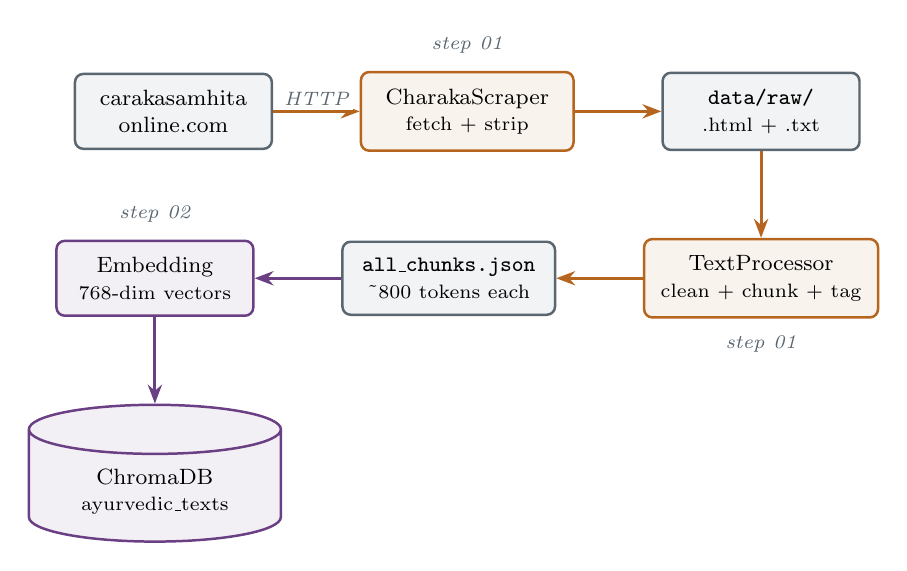
\begin{tikzpicture}[node distance=7mm]
  \node[blk=slate, minimum width=25mm, align=center] (web) {carakasamhita\\online.com};
  \node[blk=clay, right=11mm of web, minimum width=27mm, align=center] (scr) {CharakaScraper\\\scriptsize fetch + strip};
  \node[blk=slate, right=11mm of scr, minimum width=25mm, align=center] (raw) {\texttt{data/raw/}\\\scriptsize .html + .txt};
  \node[blk=clay, below=11mm of raw, minimum width=27mm, align=center] (proc) {TextProcessor\\\scriptsize clean + chunk + tag};
  \node[blk=slate, left=11mm of proc, minimum width=27mm, align=center] (chunks) {\texttt{all\_chunks.json}\\\scriptsize \textasciitilde 800 tokens each};
  \node[blk=plum, left=11mm of chunks, minimum width=25mm, align=center] (emb) {Embedding\\\scriptsize 768-dim vectors};
  \node[db=plum, below=11mm of emb, minimum width=32mm] (db) {ChromaDB\\\scriptsize ayurvedic\_texts};

  \draw[arb=clay] (web) -- node[lbl,above]{HTTP} (scr);
  \draw[arb=clay] (scr) -- (raw);
  \draw[arb=clay] (raw) -- (proc);
  \draw[arb=clay] (proc) -- (chunks);
  \draw[arb=plum] (chunks) -- (emb);
  \draw[arb=plum] (emb) -- (db);

  \node[font=\scriptsize\itshape, color=slate, above=1mm of scr] {step 01};
  \node[font=\scriptsize\itshape, color=slate, below=1mm of proc] {step 01};
  \node[font=\scriptsize\itshape, color=slate, above=1mm of emb] {step 02};
\end{tikzpicture}
\caption{Ingestion, end to end. The first three boxes run once; the Chroma collection is what the application actually queries.}
\end{figure}

\section{Scraping}

\subsection{The section table}

The eight books of the Charaka Samhita are hard-coded as a class attribute. Each entry carries a display name, the MediaWiki URL, and a Roman numeral used later as \code{section\_code} metadata.

\begin{lstlisting}[style=py,firstnumber=34]
    SECTIONS = {
        "Sutra_Sthana": {
            "name": "Section on Fundamental Principles",
            "url": "https://www.carakasamhitaonline.com/index.php?title=Sutra_Sthana",
            "code": "I"
        },
        "Nidana_Sthana": {
            "name": "Section on Diagnostic Principles",
            "url": "https://www.carakasamhitaonline.com/index.php?title=Nidana_Sthana",
            "code": "II"
        },
        # ... Vimana III, Sharira IV, Indriya V,
        #     Chikitsa VI, Kalpa VII, Siddhi VIII
    }
\end{lstlisting}

The mapping matters downstream. When a user writes ``according to the Siddhi Sthana'', the orchestrator extracts that phrase and filters retrieval on the \code{section} metadata field, which is populated from \code{name} in this table.

\begin{table}[H]
\centering
\small
\begin{tabularx}{\textwidth}{@{}c l X@{}}
\toprule
\textbf{Code} & \textbf{Sthana} & \textbf{Subject} \\
\midrule
I    & Sutra    & Fundamental principles: doshas, tastes, daily routine \\
II   & Nidana   & Diagnostics: causes and premonitory signs of disease \\
III  & Vimana   & Specific medical principles, including constitutional examination \\
IV   & Sharira  & Embryology, anatomy, formation of Prakriti at conception \\
V    & Indriya  & Prognosis read from sensory signs \\
VI   & Chikitsa & Therapeutics: disease-specific management \\
VII  & Kalpa    & Pharmaceutics: preparation of Panchakarma substances \\
VIII & Siddhi   & Procedure management and post-therapy care \\
\bottomrule
\end{tabularx}
\caption{The eight sections and what each contributes to the corpus.}
\end{table}

\subsection{Fetching}

\code{fetch\_page} is deliberately slow. It sleeps \code{REQUEST\_DELAY} seconds after every successful request and doubles that on retry, then gives up after \code{MAX\_RETRIES}. The User-Agent identifies the crawler.

\begin{lstlisting}[style=py,firstnumber=95]
    def fetch_page(self, url: str) -> Tuple[str, bool]:
        for attempt in range(self.max_retries):
            try:
                response = self.session.get(url, timeout=self.timeout)
                response.raise_for_status()
                time.sleep(self.delay)          # Be respectful to the server
                return response.text, True
            except requests.RequestException as e:
                logger.warning(f"Attempt {attempt + 1} failed for {url}: {e}")
                if attempt < self.max_retries - 1:
                    time.sleep(self.delay * 2)  # Longer delay on retry
        logger.error(f"Failed to fetch {url} after {self.max_retries} attempts")
        return "", False
\end{lstlisting}

The function returns a \code{(text, ok)} tuple rather than raising, so a single dead chapter logs a warning and the run continues. That is why a completed scrape can still be missing chapters --- check \code{total\_chapters} in \code{scraping\_summary.json} against what the site lists.

\subsection{Finding chapter links}

There is no sitemap, so chapters are discovered by scanning every anchor inside the MediaWiki content div and keeping the ones that look like article links:

\begin{lstlisting}[style=py,firstnumber=133]
        content_div = soup.find('div', {'id': 'mw-content-text'})
        if content_div:
            links = content_div.find_all('a', href=True)
            for link in links:
                href  = link.get('href', '')
                title = link.get_text(strip=True)
                # Filter for actual chapter links
                if href.startswith('/index.php?title=') and len(title) > 10:
                    if any(skip in title.lower()
                           for skip in ['main page', 'category', 'help', 'search']):
                        continue
                    chapters.append({'title': title, 'url': f"{base_url}{href}"})
\end{lstlisting}

Two heuristics carry the whole thing: the href prefix, and a link text longer than ten characters. Both are guesses about how the site is built. If carakasamhitaonline.com changes its markup, \code{extract\_chapter\_links} returns an empty list, the section directory gets an \code{index.html} and nothing else, and the run reports success. That silent failure is the most likely way a fresh scrape produces a thin corpus.

\subsection{What lands on disk}

\begin{lstlisting}[style=plain]
data/raw/
|-- scraping_summary.json          totals across all 8 sections
|-- Sutra_Sthana/
|   |-- index.html   index.txt     the section landing page
|   |-- chapter_01.html  chapter_01.txt
|   |-- chapter_02.html  chapter_02.txt
|   |-- ...
|   `-- metadata.json              per-chapter titles, URLs, word counts
|-- Nidana_Sthana/
`-- ...
\end{lstlisting}

Both HTML and plain text are kept. The text is what feeds the processor; the HTML is insurance against needing to re-extract without re-crawling.

\section{Cleaning and chunking}

\subsection{Why 800 and 200}

\code{AyurvedicTextProcessor} defaults to 800-token chunks with 200 tokens of overlap, counted with \code{tiktoken}'s \code{cl100k\_base} encoding. Eight hundred tokens is roughly two or three verses plus their commentary --- enough that a retrieved passage carries its own explanation. The 200-token overlap means a statement that straddles a boundary still appears whole in one of the two neighbouring chunks.

\begin{figure}[H]
\centering
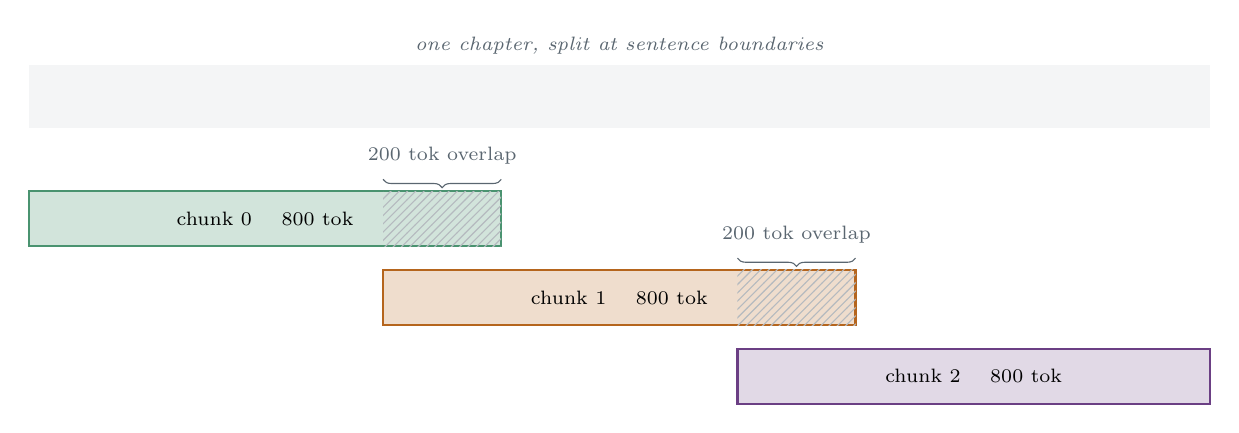
\begin{tikzpicture}[x=1mm,y=1mm]
  % chapter bar
  \fill[palegrey] (0,27) rectangle (150,35);
  \node[font=\scriptsize\itshape,color=slate] at (75,37.5) {one chapter, split at sentence boundaries};

  % chunk 1
  \fill[midgreen!25, draw=midgreen, line width=0.8pt] (0,12) rectangle (60,19);
  \node[font=\scriptsize] at (30,15.5) {chunk 0 \quad 800 tok};
  % chunk 2
  \fill[clay!22, draw=clay, line width=0.8pt] (45,2) rectangle (105,9);
  \node[font=\scriptsize] at (75,5.5) {chunk 1 \quad 800 tok};
  % chunk 3
  \fill[plum!20, draw=plum, line width=0.8pt] (90,-8) rectangle (150,-1);
  \node[font=\scriptsize] at (120,-4.5) {chunk 2 \quad 800 tok};

  % overlap braces
  \draw[decorate,decoration={brace,amplitude=3pt},color=slate] (60,20.5) -- (45,20.5);
  \node[font=\scriptsize,color=slate] at (52.5,23.5) {200 tok overlap};
  \draw[decorate,decoration={brace,amplitude=3pt},color=slate] (105,10.5) -- (90,10.5);
  \node[font=\scriptsize,color=slate] at (97.5,13.5) {200 tok overlap};

  % overlap hatch
  \fill[pattern=north east lines, pattern color=slate!45] (45,12) rectangle (60,19);
  \fill[pattern=north east lines, pattern color=slate!45] (90,2) rectangle (105,9);
\end{tikzpicture}
\vspace{4mm}
\caption{The overlap window. Hatched regions are duplicated between neighbouring chunks, so a sentence never falls into the gap between two retrievable passages.}
\end{figure}

\subsection{The chunking loop}

Text is split into sentences with a lookbehind regex, then sentences are accumulated until the token budget is hit. The interesting part is what happens at the boundary --- the loop walks backwards through the chunk it just closed, collecting whole sentences until it has 200 tokens of context, and seeds the next chunk with them.

\begin{lstlisting}[style=py,firstnumber=134]
        # Split into sentences
        sentences = re.split(r'(?<=[.!?])\s+', text)

        current_chunk  = []
        current_tokens = 0
        chunk_id       = 0

        for sentence in sentences:
            sentence = sentence.strip()
            if not sentence:
                continue

            sentence_tokens = self.count_tokens(sentence)

            # Check if adding this sentence exceeds chunk size
            if current_tokens + sentence_tokens > self.chunk_size and current_chunk:
                chunks.append({
                    'chunk_id':    chunk_id,
                    'text':        ' '.join(current_chunk),
                    'token_count': current_tokens,
                    'metadata':    metadata.copy()
                })
                chunk_id += 1

                # Start new chunk with overlap: keep trailing sentences
                overlap_sentences, overlap_tokens = [], 0
                for sent in reversed(current_chunk):
                    sent_tokens = self.count_tokens(sent)
                    if overlap_tokens + sent_tokens <= self.chunk_overlap:
                        overlap_sentences.insert(0, sent)
                        overlap_tokens += sent_tokens
                    else:
                        break

                current_chunk  = overlap_sentences
                current_tokens = overlap_tokens

            current_chunk.append(sentence)
            current_tokens += sentence_tokens
\end{lstlisting}

Because overlap is measured in whole sentences, the actual overlap is usually a little under 200 tokens --- the loop stops as soon as the next sentence backwards would exceed the budget. A chunk is never split mid-sentence, which is the point.

\begin{warn}[title={The sentence splitter and Sanskrit transliteration}]
\code{re.split(r'(?<=[.!?])\textbackslash s+', text)} treats every period as a sentence end. Transliterated Sanskrit and the site's verse numbering (``Ch.~Su.~1.42'') contain periods that are not sentence boundaries, so some chunks begin mid-citation. The overlap window softens this but does not eliminate it.
\end{warn}

\subsection{Cleaning}

\code{clean\_text} runs before chunking and does four things: collapses runs of three or more newlines to two, collapses multiple spaces to one, deletes \code{[Page N]} markers and bare numeric lines, and normalises curly quotes to straight ones.

\begin{lstlisting}[style=py,firstnumber=69]
        text = re.sub(r'\n\s*\n\s*\n', '\n\n', text)
        text = re.sub(r'  +', ' ', text)
        text = re.sub(r'\[Page \d+\]', '', text)
        text = re.sub(r'^\d+\s*$', '', text, flags=re.MULTILINE)
\end{lstlisting}

\section{Metadata: the four keys everything depends on}

Each chunk carries a metadata dictionary. Four keys are load-bearing:

\begin{table}[H]
\centering
\small
\begin{tabularx}{\textwidth}{@{}l l X@{}}
\toprule
\textbf{Key} & \textbf{Example} & \textbf{Used for} \\
\midrule
\code{section} & \code{"Section on Therapeutic Principles"} & Source filtering when a user names a Sthana; printed in every citation \\
\code{section\_code} & \code{"VI"} & Not queried, kept for reference \\
\code{chapter} & \code{"Jvara Chikitsa"} & Second half of every citation line \\
\code{category} & \code{"treatment"} & \textbf{The agent routing key.} Each specialist filters on exactly one value \\
\bottomrule
\end{tabularx}
\caption{Chunk metadata. \code{category} is what makes the three agents see three different corpora.}
\end{table}

\subsection{How categories are assigned}
\label{sec:categorise}

\code{categorize\_content} is a keyword cascade over the lowercased chunk text, with a fall-through to section-based assignment:

\begin{lstlisting}[style=py,firstnumber=226]
        text_lower = text.lower()

        # Prakriti-related content
        if any(term in text_lower for term in
               ['vata', 'pitta', 'kapha', 'constitution', 'prakriti']):
            return 'prakriti'

        # Vikriti/Disease content
        if any(term in text_lower for term in
               ['disease', 'symptom', 'disorder', 'imbalance', 'dosha']):
            return 'vikriti'

        # Treatment content
        if any(term in text_lower for term in
               ['treatment', 'therapy', 'remedy', 'herb', 'diet', 'lifestyle']):
            return 'treatment'

        # Default to section-based categorization
        if 'chikitsa' in section_name.lower():
            return 'treatment'
        elif 'nidana' in section_name.lower() or 'vimana' in section_name.lower():
            return 'vikriti'
        else:
            return 'general'
\end{lstlisting}

Order decides everything, and the order is not neutral. The three dosha names are in the first test, and the three dosha names appear on a large share of pages in any Ayurvedic text. A passage from the Chikitsa Sthana that reads ``for aggravated Vata, administer Basti'' contains \code{vata} and so is tagged \code{prakriti} --- not \code{treatment} --- even though it is a treatment instruction sitting in the therapeutics book. The treatment agent, which filters on \code{category == "treatment"}, will never retrieve it.

\begin{bug}[title={Consequence: the treatment corpus is smaller than it looks}]
Because \code{prakriti} is tested first and its keywords are the most common words in the corpus, the \code{prakriti} bucket absorbs passages that belong to the other two agents. Run the category breakdown printed at the end of step 1 and check the split before drawing conclusions about agent quality. A more balanced assignment would score all three keyword sets and pick the highest, or tag chunks with multiple categories and use Chroma's \code{\$in} operator at query time.
\end{bug}

\section{Output of the processing stage}

\code{process\_all()} writes two files. \code{all\_chunks.json} is a flat list of every chunk:

\begin{lstlisting}[style=json]
[
  {
    "chunk_id": 0,
    "text": "Vata is characterised by the qualities ruksha, laghu, sheeta ...",
    "token_count": 782,
    "metadata": {
      "section":        "Section on Fundamental Principles",
      "section_code":   "I",
      "chapter":        "Deerghanjiviteeya Adhyaya",
      "chapter_number": 1,
      "source_url":     "https://www.carakasamhitaonline.com/index.php?title=...",
      "source_file":    "chapter_01.txt",
      "source_path":    "data/raw/Sutra_Sthana/chapter_01.txt",
      "category":       "prakriti"
    }
  }
]
\end{lstlisting}

\code{processing\_summary.json} holds the totals, the per-section chunk and token counts, and the category histogram. The README estimates 5,000--8,000 chunks for the full corpus.

\chapter{The Retrieval Layer}

Three small classes sit between a question and the passages that answer it. \code{EmbeddingGenerator} turns text into vectors, \code{AyurvedicVectorStore} owns the Chroma collection, and \code{RAGRetriever} joins them. Together they are under 130 lines. No framework is involved --- despite \code{langchain} being pinned in \fpath{requirements.txt}, it is never imported.

\begin{figure}[H]
\centering
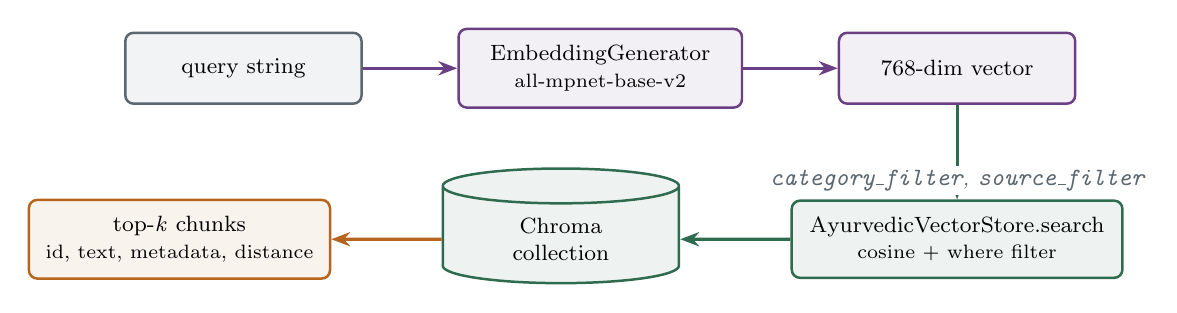
\begin{tikzpicture}[node distance=8mm]
  \node[blk=slate, minimum width=30mm] (q) {query string};
  \node[blk=plum, right=12mm of q, minimum width=36mm, align=center]
       (e) {EmbeddingGenerator\\\scriptsize all-mpnet-base-v2};
  \node[blk=plum, right=12mm of e, minimum width=30mm, align=center]
       (v) {768-dim vector};
  \node[blk=deepgreen, below=12mm of v, minimum width=42mm, align=center]
       (s) {AyurvedicVectorStore.search\\\scriptsize cosine + where filter};
  \node[db=deepgreen, left=14mm of s, minimum width=30mm] (c) {Chroma\\collection};
  \node[blk=clay, left=14mm of c, minimum width=34mm, align=center]
       (r) {top-\emph{k} chunks\\\scriptsize id, text, metadata, distance};

  \draw[arb=plum] (q) -- (e);
  \draw[arb=plum] (e) -- (v);
  \draw[arb=deepgreen] (v) -- (s);
  \draw[arb=deepgreen] (s) -- (c);
  \draw[arb=clay] (c) -- (r);

  \node[lbl, above=0.5mm of s] {\code{category\_filter}, \code{source\_filter}};
\end{tikzpicture}
\caption{One retrieval. The two filters are optional and are combined into a single Chroma \code{where} clause.}
\end{figure}

\section{Embeddings}

\begin{lstlisting}[style=py]
class EmbeddingGenerator:
    def __init__(self, model_name: str = None):
        if model_name is None:
            model_name = os.getenv("EMBEDDING_MODEL",
                                   "sentence-transformers/all-mpnet-base-v2")
        self.model = SentenceTransformer(model_name)
        self.embedding_dim = self.model.get_sentence_embedding_dimension()

    def embed_text(self, text: str) -> np.ndarray:
        return self.model.encode(text, convert_to_numpy=True)

    def embed_batch(self, texts: List[str], batch_size: int = 32) -> np.ndarray:
        return self.model.encode(texts, batch_size=batch_size,
                                 show_progress_bar=True, convert_to_numpy=True)
\end{lstlisting}

\code{all-mpnet-base-v2} produces 768-dimensional vectors and is a general-purpose English model. It has never seen Sanskrit, so transliterated terms are embedded as unfamiliar token sequences. Retrieval works because the scraped text is an English translation with Sanskrit terms interleaved --- the English carries the semantic signal. Queries written mostly in transliterated Sanskrit will retrieve worse than the same question asked in English.

The class is instantiated twice in a normal session: once by \fpath{scripts/02\_build\_vectordb.py} to embed the corpus, once by \code{AyurMindApp} to embed queries. Both load the same model weights, roughly 420~MB, into memory.

\begin{note}[title={Why \code{embed\_batch} exists separately}]
Indexing embeds thousands of chunks at once, which is far faster in batches of 32 with a progress bar. Query time embeds exactly one string, where the batching machinery is pure overhead. Hence two methods over the same model.
\end{note}

\section{The vector store}

\code{AyurvedicVectorStore} wraps a single persistent Chroma collection.

\begin{lstlisting}[style=py,firstnumber=9]
    def __init__(self, persist_directory: str = None):
        if persist_directory is None:
            persist_directory = os.getenv("VECTOR_DB_PATH", "./data/vectordb")
        self.persist_directory = Path(persist_directory)
        self.persist_directory.mkdir(parents=True, exist_ok=True)

        self.client = chromadb.PersistentClient(path=str(self.persist_directory))
        self.collection = self.client.get_or_create_collection(
            name="ayurvedic_texts",
            metadata={"description": "Charaka Samhita chunks"}
        )
\end{lstlisting}

\code{get\_or\_create\_collection} makes the constructor safe to call against an empty directory --- you get an empty collection rather than an exception. That is convenient and also the reason a misconfigured \code{VECTOR\_DB\_PATH} produces zero search results instead of a clear error.

\subsection{Indexing}

\begin{lstlisting}[style=py,firstnumber=21]
    def add_chunks(self, chunks: List[Dict], embeddings: List[List[float]],
                   batch_size: int = 100):
        for i in tqdm(range(0, len(chunks), batch_size), desc="Adding chunks"):
            batch_chunks     = chunks[i:i+batch_size]
            batch_embeddings = embeddings[i:i+batch_size]

            ids       = [f"chunk_{i+j}" for j in range(len(batch_chunks))]
            documents = [chunk['text']     for chunk in batch_chunks]
            metadatas = [chunk['metadata'] for chunk in batch_chunks]

            self.collection.add(ids=ids, documents=documents,
                                embeddings=batch_embeddings, metadatas=metadatas)
\end{lstlisting}

IDs are positional --- \code{chunk\_0} through \code{chunk\_N}, derived from the offset in \code{all\_chunks.json}. They carry no meaning and are not stable across rebuilds: re-running the scraper with a different chapter count renumbers everything. Nothing in the application relies on ID stability, but the evaluation results files record source IDs, so those IDs only make sense against the database version they were produced with.

\begin{warn}[title={Re-indexing does not clear the collection}]
\code{add\_chunks} only calls \code{collection.add}. Running \fpath{scripts/02\_build\_vectordb.py} twice against an existing database attempts to insert the same IDs again. Delete \code{data/vectordb/} before a rebuild.
\end{warn}

\subsection{Search and the where clause}

This is the most consequential method in the retrieval layer, because it is where the agents' category filters and the orchestrator's source filter get combined.

\begin{lstlisting}[style=py,firstnumber=32]
    def search(self, query_embedding: List[float], n_results: int = 5,
               category_filter: Optional[str] = None,
               source_filter:   Optional[str] = None) -> Dict:
        where_conditions = []
        if category_filter:
            where_conditions.append({"category": category_filter})

        if source_filter:
            # Match source_filter against 'section' or 'chapter' metadata
            where_conditions.append({"$or": [{"section": source_filter},
                                             {"chapter":  source_filter}]})

        where_clause = None
        if where_conditions:
            if len(where_conditions) == 1:
                where_clause = where_conditions[0]
            else:
                where_clause = {"$and": where_conditions}

        return self.collection.query(query_embeddings=[query_embedding],
                                     n_results=n_results, where=where_clause)
\end{lstlisting}

Three shapes come out of that logic:

\begin{lstlisting}[style=json]
// no filters - the fast path and unfiltered helper calls
where = None

// category only - the normal case for every specialist agent
where = {"category": "treatment"}

// category + source - user named a Sthana in the query
where = {"$and": [
           {"category": "treatment"},
           {"$or": [{"section": "Siddhi Sthana"},
                    {"chapter":  "Siddhi Sthana"}]}
         ]}
\end{lstlisting}

\begin{bug}[title={The source filter needs an exact string match}]
Chroma's \code{where} does equality, not substring matching. The \code{section} values written by the processor are full display names --- \code{"Section on Therapeutic Procedures"} --- while the orchestrator's regex extracts \code{"Siddhi Sthana"}. Those strings are not equal, so the \code{\$or} matches nothing, the \code{\$and} matches nothing, and a query that names a Sthana retrieves \textbf{zero} chunks rather than more focused ones. Fixing this means either storing the Sthana key (\code{"Siddhi\_Sthana"} $\rightarrow$ \code{"Siddhi Sthana"}) as its own metadata field, or mapping the extracted phrase to the full display name before filtering.
\end{bug}

\subsection{Statistics}

\begin{lstlisting}[style=py,firstnumber=51]
    def get_stats(self) -> Dict:
        total_count = self.collection.count()
        return {'total_chunks': total_count, 'categories': {}}
\end{lstlisting}

\code{categories} is a placeholder that always returns empty. The real category histogram is in \code{data/processed/processing\_summary.json}, written during step 1.

\section{The retriever}

\code{RAGRetriever} owns the default result count and reshapes Chroma's column-oriented response into a list of dictionaries.

\begin{lstlisting}[style=py,firstnumber=13]
    def retrieve(self, query: str, n_results: int = None,
                 category_filter: Optional[str] = None,
                 source_filter:   Optional[str] = None) -> List[Dict]:
        if n_results is None:
            n_results = self.max_chunks          # MAX_CHUNKS_PER_QUERY, default 5

        query_embedding = self.embedding_generator.embed_text(query)
        results = self.vectorstore.search(
            query_embedding=query_embedding.tolist(), n_results=n_results,
            category_filter=category_filter, source_filter=source_filter)

        retrieved_chunks = []
        for i in range(len(results['ids'][0])):
            retrieved_chunks.append({
                'id':       results['ids'][0][i],
                'text':     results['documents'][0][i],
                'metadata': results['metadatas'][0][i],
                'distance': results['distances'][0][i]
                            if 'distances' in results else None
            })
        return retrieved_chunks
\end{lstlisting}

The \code{[0]} indexing everywhere is Chroma's batch dimension --- \code{query} accepts a list of query vectors and returns parallel lists of results. One query goes in, so index zero comes out.

Note what is \emph{not} here: no distance threshold, no reranking, no deduplication, no minimum-relevance cutoff. Whatever the nearest five vectors are, they go into the prompt. If the collection holds nothing relevant, the five least-irrelevant chunks are still retrieved and still presented to the model as authoritative context. This is the main structural weakness of the grounding story, and it is worth knowing when reading the hallucination-rate discussion in Chapter~\ref{ch:eval}.

\subsection{Two ways to build context}

\code{RAGRetriever.build\_context()} formats chunks into a prompt-ready string. It is used by the single-agent RAG baseline in the evaluation harness:

\begin{lstlisting}[style=py,firstnumber=32]
    def build_context(self, query: str, n_results: int = None,
                      category_filter: Optional[str] = None,
                      include_metadata: bool = True) -> str:
        chunks = self.retrieve(query, n_results, category_filter)
        context_parts = []
        for i, chunk in enumerate(chunks, 1):
            if include_metadata:
                metadata = chunk['metadata']
                source = (f"[Source: {metadata.get('section', 'Unknown')} - "
                          f"{metadata.get('chapter', 'Unknown')}]")
                context_parts.append(f"--- Context {i} {source} ---")
            else:
                context_parts.append(f"--- Context {i} ---")
            context_parts.append(chunk['text'])
            context_parts.append("")
        return "\n".join(context_parts)
\end{lstlisting}

The agents do not call it. \code{BaseAgent.retrieve\_context\_and\_sources()} produces the same string but also returns the raw chunk list, because the orchestrator needs the chunk metadata to build its citation block. The duplication is small but real: two functions format context identically, and \code{build\_context} has no \code{source\_filter} parameter, so it cannot honour a user's request for a specific Sthana.

The resulting context string looks like this:

\begin{lstlisting}[style=plain]
--- Context 1 [Source: Section on Therapeutic Principles - Jvara Chikitsa] ---
In the management of Jvara, the physician should first assess the state of
Agni. Langhana is indicated in Ama-avastha ...

--- Context 2 [Source: Section on Fundamental Principles - Deerghanjiviteeya] ---
...
\end{lstlisting}

\chapter{The Language Model Layer}

Four client classes live in \fpath{src/llm/}. They target different APIs but expose the same two methods, so any of them can be dropped into an agent without the agent knowing which one it got.

\section{The informal interface}

There is no abstract base class here --- the contract is duck-typed. Every client implements:

\begin{lstlisting}[style=py]
def generate(self, prompt: str,
             system_prompt: Optional[str] = None,
             temperature: float = ...,
             max_tokens: int = ...,
             conversation_history: Optional[List[Dict]] = None,
             **kwargs) -> str

def generate_with_context(self, query: str, context: str,
                          system_prompt: str,
                          temperature: float = ...,
                          max_tokens: int = ...,
                          conversation_history: Optional[List[Dict]] = None) -> str
\end{lstlisting}

\code{generate\_with\_context} is the RAG entry point and is the same in all four files --- it wraps the retrieved passages and the question in a fixed template, then delegates to \code{generate}:

\begin{lstlisting}[style=py]
        prompt = f"""Context from Ayurvedic texts:

{context}

---

User Query: {query}

Based on the context provided above, please provide a response."""
\end{lstlisting}

Specialist agents call \code{generate\_with\_context}. The orchestrator calls \code{generate} directly, both for the fast path and for synthesis, because by then the context has already been consumed and what it is passing along is the specialists' prose.

\section{The four clients side by side}

\begin{table}[H]
\centering
\small
\begin{tabularx}{\textwidth}{@{}l l l X@{}}
\toprule
\textbf{Client} & \textbf{Default model} & \textbf{Selected by} & \textbf{Notes} \\
\midrule
\code{GoogleClient} & \code{gemini-1.5-flash} & fallback, always last & The de facto default. \code{google-generativeai} SDK, stateless \code{generate\_content}. \\
\addlinespace
\code{OpenAIClient} & \code{gpt-4o-mini} & \code{USE\_OPENAI=true} & \code{openai} SDK. Thinnest of the four at 74 lines. \\
\addlinespace
\code{OllamaClient} & \code{llama3.2:3b} & \code{USE\_LOCAL\_LLM=true} & Raw HTTP to \code{localhost:11434}. Free and offline; ignores \code{max\_tokens}. \\
\addlinespace
\code{OpenRouterClient} & \code{mistral-7b-instruct:free} & \textbf{never} & Raw HTTP. Not imported anywhere in the application. \\
\bottomrule
\end{tabularx}
\caption{Client comparison. Only the first three are reachable from the running application.}
\end{table}

\section{Provider selection}

\code{AyurMindApp.\_\_init\_\_} walks a fixed preference order, catching failures at each step:

\begin{figure}[H]
\centering
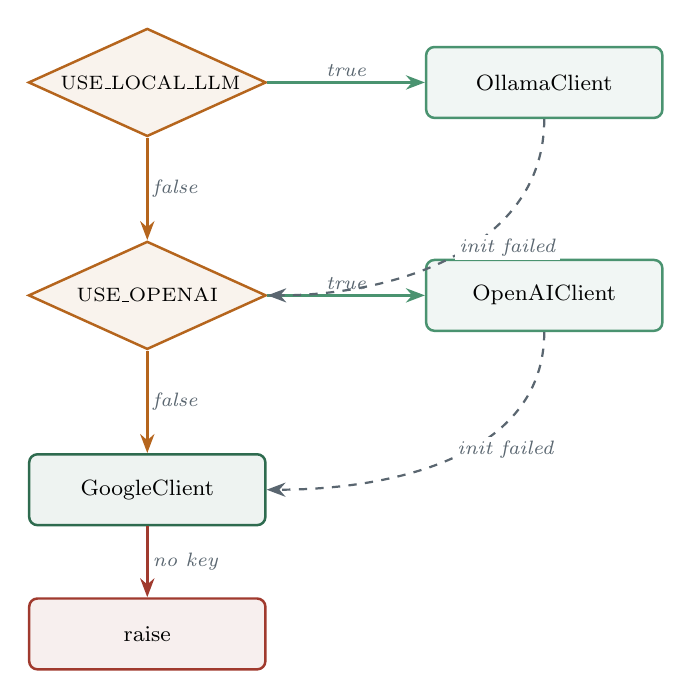
\begin{tikzpicture}[node distance=7mm]
  \node[dia=clay, text width=22mm] (d1) {USE\_LOCAL\_LLM};
  \node[blk=midgreen, right=20mm of d1, minimum width=30mm] (ol) {OllamaClient};
  \node[dia=clay, below=13mm of d1, text width=22mm] (d2) {USE\_OPENAI};
  \node[blk=midgreen, right=20mm of d2, minimum width=30mm] (oa) {OpenAIClient};
  \node[blk=deepgreen, below=13mm of d2, minimum width=30mm] (gg) {GoogleClient};
  \node[blk=brick, below=9mm of gg, minimum width=30mm] (er) {raise};

  \draw[arb=midgreen] (d1) -- node[lbl,above]{true} (ol);
  \draw[arb=clay] (d1) -- node[lbl,right]{false} (d2);
  \draw[arb=midgreen] (d2) -- node[lbl,above]{true} (oa);
  \draw[arb=clay] (d2) -- node[lbl,right]{false} (gg);
  \draw[arb=brick] (gg) -- node[lbl,right]{no key} (er);

  \draw[ar, dashed] (ol.south) to[out=-90,in=0] node[lbl,right,yshift=1mm]{init failed} (d2.east);
  \draw[ar, dashed] (oa.south) to[out=-90,in=0] node[lbl,right,yshift=1mm]{init failed} (gg.east);
\end{tikzpicture}
\caption{Fallback chain. A client that raises during construction is logged as a warning and the next option is tried; only a Google failure is fatal.}
\end{figure}

\begin{lstlisting}[style=py,firstnumber=48]
        self.llm_client = None
        use_local_llm = os.getenv("USE_LOCAL_LLM", "false").lower() == "true"
        use_openai    = os.getenv("USE_OPENAI",    "false").lower() == "true"

        if use_local_llm:
            try:
                self.llm_client = OllamaClient()
                app_logger.info(f"Using Local client: {self.llm_client.model_name}")
            except Exception as e:
                app_logger.warning(f"Local LLM Client failed: {e}. Falling back.")

        if self.llm_client is None and use_openai:
            try:
                self.llm_client = OpenAIClient()
                app_logger.info(f"Using OpenAI client: {self.llm_client.model_name}")
            except Exception as e:
                app_logger.warning(f"OpenAI Client failed: {e}. Falling back to Google.")

        if self.llm_client is None:
            try:
                self.llm_client = GoogleClient()
                app_logger.info(f"Using Google client: {self.llm_client.model_name}")
            except Exception as e:
                app_logger.error(f"Failed to initialize GoogleClient: {e}.")
                raise e     # Critical failure if no client can be initialized
\end{lstlisting}

The fallback covers construction only. Once a client is chosen, a mid-session API error propagates up to the Gradio handler and is shown as an error message in the chat; there is no runtime failover to a second provider.

Note also that \code{OllamaClient.\_\_init\_\_} does not raise when Ollama is unreachable --- it logs a warning and returns a usable object. So \code{USE\_LOCAL\_LLM=true} with Ollama stopped selects the Ollama client successfully and then fails on the first generation call, rather than falling through to OpenAI or Google.

\section{Conversation history handling}

All four clients accept a \code{conversation\_history} list of \code{\{"role", "content"\}} dictionaries, and this is where their behaviour genuinely diverges.

\subsection{Google}

Gemini names the assistant role \code{model}, so history is remapped. The client also has to cope with Gradio's message format, where \code{content} can be a list of part-dictionaries rather than a plain string:

\begin{lstlisting}[style=py,firstnumber=62]
    def _format_history(self, conversation_history):
        if not conversation_history:
            return []
        formatted_history = []
        for turn in conversation_history:
            # Gemini uses 'model' for the assistant's role, 'user' for user
            role = "model" if turn["role"] == "assistant" else "user"
            text_content = self._extract_text_content(turn["content"])
            formatted_history.append({"role": role, "parts": [text_content]})
        return formatted_history
\end{lstlisting}

\code{\_extract\_text\_content} handles four shapes --- a plain string, a list of dicts with \code{text} keys, a single dict with a \code{text} key, and anything else via \code{str()}. That defensiveness exists because Gradio has changed its chat message schema more than once.

\subsection{OpenRouter and Ollama drop the last turn}

Both slice the history before using it:

\begin{lstlisting}[style=py]
        # OpenRouterClient.generate
        if conversation_history:
            # Add all but the last user message from history
            for turn in conversation_history[:-1]:
                messages.append(turn)
\end{lstlisting}

That slice is correct for how the UI calls them. \code{AyurMindApp.chat()} appends the user's new message to \code{history} \emph{before} passing it down, so the last element of \code{conversation\_history} is the same message that arrives separately as \code{prompt}.

\begin{bug}[title={Google and OpenAI send the current message twice}]
\code{GoogleClient.\_format\_history} iterates the whole list, then appends the prompt on top. \code{OpenAIClient} does the same. Since the UI has already appended the user's message to \code{history}, the model receives it once verbatim from history and again wrapped in the RAG or synthesis prompt. With the default Google client this happens on every slow-path turn --- once per specialist agent plus once for synthesis. Adding \code{[:-1]} in both clients, matching the OpenRouter and Ollama behaviour, resolves it.
\end{bug}

\subsection{Ollama flattens history into the prompt}

The Ollama \code{/api/generate} endpoint takes one string, so the client builds the transcript by hand:

\begin{lstlisting}[style=py,firstnumber=66]
        full_prompt = ""
        if system_prompt:
            full_prompt += f"{system_prompt}\n\n"
        if history_str:
            full_prompt += f"Previous conversation:\n{history_str}\n"
        full_prompt += f"Current query: {prompt}"

        payload = {
            "model": self.model,
            "prompt": full_prompt,
            "stream": False,
            "options": {"temperature": temperature,
                        "num_predict": 800}      # Ollama's max_tokens equivalent
        }
\end{lstlisting}

\code{num\_predict} is fixed at 800 regardless of what the caller asked for, and \code{max\_tokens} is popped from \code{kwargs} and discarded. Agents request 3000 tokens and the orchestrator requests 4000; against Ollama they all get 800. That truncation explains a great deal about the local-model evaluation outputs in Chapter~\ref{ch:eval} --- the four-section report the synthesis prompt asks for does not fit in 800 tokens.

\section{Error handling}

\code{OpenRouterClient} is the only one that translates HTTP status codes into actionable messages:

\begin{lstlisting}[style=py,firstnumber=70]
        except requests.exceptions.HTTPError as e:
            status_code = e.response.status_code
            if status_code == 401:
                raise RuntimeError("OpenRouter API Error: Invalid API Key. ...")
            elif status_code == 402:
                raise RuntimeError("OpenRouter API Error: You have exceeded "
                                   "your free tier limit or credits.")
            elif status_code == 404:
                raise RuntimeError(f"OpenRouter API Error: Model '{self.model}' "
                                   "not found. ...")
\end{lstlisting}

The other three wrap everything in a single \code{RuntimeError} carrying the original exception text. Google additionally treats an empty \code{response.text} as an error, which catches the case where Gemini's safety filters block a generation and return a response with no candidates --- a realistic outcome when the prompt describes symptoms and asks for treatment.

\begin{lstlisting}[style=py,firstnumber=142]
            if not response.text:
                raise ValueError("Empty response from model")
\end{lstlisting}

\section{Timeouts}

Both HTTP clients use 180 seconds. That is generous, and deliberately so: the slow path can issue four sequential generations, and a 3B model on CPU is not fast.

\begin{table}[H]
\centering
\small
\begin{tabular}{@{}l l l@{}}
\toprule
\textbf{Client} & \textbf{Timeout} & \textbf{Set where} \\
\midrule
\code{OpenRouterClient} & 180~s & \code{requests.post(..., timeout=180)} \\
\code{OllamaClient} & 180~s generate, 2~s availability probe & \code{is\_available()} uses the short one \\
\code{GoogleClient} & SDK default & not overridden \\
\code{OpenAIClient} & SDK default & not overridden \\
\bottomrule
\end{tabular}
\caption{Timeout settings. A full slow-path consultation can legitimately take several minutes.}
\end{table}

\chapter{The Agent Layer}
\label{ch:agents}

This is where the design lives. Four classes: one abstract base, three specialists that differ only in a prompt and a filter, and an orchestrator that has all the control flow.

\section{BaseAgent: the template}

\code{BaseAgent} is 63 lines and defines the entire agent contract through two abstract methods and one concrete pipeline.

\begin{lstlisting}[style=py,firstnumber=5]
class BaseAgent(ABC):
    def __init__(self, name: str, rag_retriever, llm_client,
                 temperature: float = 0.3, max_tokens: int = 3000):
        self.name          = name
        self.rag_retriever = rag_retriever
        self.llm_client    = llm_client
        self.temperature   = temperature
        self.max_tokens    = max_tokens

    @abstractmethod
    def get_system_prompt(self) -> str: ...

    @abstractmethod
    def get_category_filter(self) -> Optional[str]: ...
\end{lstlisting}

A subclass supplies a personality (the system prompt) and a slice of the corpus (the category filter). Everything else is inherited. Adding a fourth specialist is therefore a 15-line file --- see Chapter~\ref{ch:extend}.

\subsection{process(): the three-step pipeline}

\begin{lstlisting}[style=py,firstnumber=59]
    def process(self, query: str, additional_info: Dict = None,
                conversation_history: list = None) -> Dict:
        source_filter = additional_info.get('source_filter') if additional_info else None
        context, sources = self.retrieve_context_and_sources(query, source_filter=source_filter)
        response = self.generate_response(query, context, additional_info, conversation_history)
        return {'agent': self.name, 'response': response,
                'sources': sources, 'query': query}
\end{lstlisting}

Retrieve, generate, return both the prose and the chunks it came from. Returning \code{sources} alongside \code{response} is what lets the orchestrator build a citation list without re-running retrieval.

\subsection{Retrieval with the agent's own filter}

\begin{lstlisting}[style=py,firstnumber=21]
    def retrieve_context_and_sources(self, query: str, n_results: int = 5,
                                     source_filter: Optional[str] = None):
        category_filter = self.get_category_filter()
        chunks = self.rag_retriever.retrieve(query=query, n_results=n_results,
                                             category_filter=category_filter,
                                             source_filter=source_filter)
        context_parts = []
        for i, chunk in enumerate(chunks, 1):
            metadata = chunk.get('metadata', {})
            source = (f"[Source: {metadata.get('section', 'Unknown')} - "
                      f"{metadata.get('chapter', 'Unknown')}]")
            context_parts.append(f"--- Context {i} {source} ---")
            context_parts.append(chunk.get('text', ''))
            context_parts.append("")
        return "\n".join(context_parts), chunks
\end{lstlisting}

The category filter comes from the subclass and is never overridden by the caller. That is the mechanism behind the whole multi-agent premise: three agents asking the same corpus the same question get three different answers because each one is only allowed to see a third of it.

\subsection{Passing structured findings between agents}

\code{generate\_response} folds an \code{additional\_info} dictionary into the query as labelled lines, after removing the one key that is meant for retrieval rather than for the model:

\begin{lstlisting}[style=py,firstnumber=43]
        # Ensure 'source_filter' is not included in the LLM's additional_info
        llm_additional_info = additional_info.copy() if additional_info else {}
        llm_additional_info.pop('source_filter', None)

        if llm_additional_info:
            info_str = "\n".join([f"{key}: {value}"
                                  for key, value in llm_additional_info.items()])
            enhanced_query = f"{query}\n\nAdditional Information:\n{info_str}"
        else:
            enhanced_query = query
\end{lstlisting}

So the treatment agent's actual query text ends up looking like:

\begin{lstlisting}[style=plain]
I have acid reflux and skin rashes. What should I do?

Additional Information:
Prakriti: **Provisional Constitutional Assessment**: Pitta-dominant, high confidence.
  The user's ...
Dosha Imbalance: **Provisional Diagnosis (Vikriti Nirnaya)**: Pitta Prakopa with
  Tikshnagni. Amlapitta is indicated by ...
\end{lstlisting}

Prose is passed between agents, not structured data. There is no schema, no parsing, no validation --- the downstream agent reads its predecessor's report the way a junior clinician reads a colleague's notes. That keeps the code short and makes the handoff lossy in a way that is hard to measure.

\begin{note}[title={One retrieval too many}]
\code{process()} calls \code{retrieve\_context\_and\_sources()} and then passes the resulting context into \code{generate\_response()}. But \code{generate\_response()} also retrieves when \code{context is None}, so it carries a second, unreachable retrieval path. The dead branch is harmless; it just means two functions know how to fetch context.
\end{note}

\section{The three specialists}

\begin{table}[H]
\centering
\small
\begin{tabularx}{\textwidth}{@{}l l c l X@{}}
\toprule
\textbf{Class} & \textbf{\code{name}} & \textbf{Temp} & \textbf{Filter} & \textbf{Persona in the system prompt} \\
\midrule
\code{PrakritiAgent} & Prakriti Assessor & 0.3 & \code{prakriti} & Senior professor of Sharira Vijnana \\
\code{DoshaAgent} & Dosha Imbalance Detector & 0.3 & \code{vikriti} & Senior clinician in Vikriti Vijnana \\
\code{TreatmentAgent} & Treatment Recommender & 0.4 & \code{treatment} & Senior physician designing Chikitsa Krama \\
\bottomrule
\end{tabularx}
\caption{The three specialists. Diagnosis runs cooler than therapy design, which is given slightly more latitude at 0.4.}
\end{table}

Each class is under 40 lines and most of that is the prompt string. The whole of \fpath{src/agents/prakriti\_agent.py} outside the prompt:

\begin{lstlisting}[style=py]
class PrakritiAgent(BaseAgent):
    def __init__(self, rag_retriever, llm_client):
        super().__init__(name="Prakriti Assessor", rag_retriever=rag_retriever,
                         llm_client=llm_client, temperature=0.3)

    def get_system_prompt(self) -> str:
        return """You are a senior Ayurvedic professor specializing in ..."""

    def get_category_filter(self) -> Optional[str]:
        return "prakriti"
\end{lstlisting}

\subsection{What each prompt demands}

The prompts are the specification, so they are worth reading closely. All three share four instructions --- scholarly tone, classical citation, Sanskrit terminology with parenthetical glosses, and a fixed output structure --- and then diverge on what they must produce.

\textbf{Prakriti Assessor} must return a constitutional call with a confidence level, a per-dosha breakdown naming the specific Gunas, and a trait-to-Guna correlation table. The prompt supplies the table format inline:

\begin{lstlisting}[style=plain]
| User Trait  | Assessed Dosha | Corresponding Guna |
|-------------|----------------|--------------------|
| Dry Skin    | Vata           | Ruksha (Dry)       |
| Irritability| Pitta          | Tikshna (Sharp)    |
\end{lstlisting}

\textbf{Dosha Imbalance Detector} must go past naming a dosha and describe the pathogenesis: the nature of the vitiation (\emph{Vata Prakopa}, \emph{Pitta Kshaya}), which tissues and channels are involved (\emph{Dhatus}, \emph{Srotas}), and the state of the digestive fire (\emph{Mandagni}, \emph{Tikshnagni}).

\textbf{Treatment Recommender} has the longest prompt and the only safety-critical clause. It is instructed to lead with the treatment principle, then split recommendations into purification and palliative care, and it carries a mandatory string:

\begin{lstlisting}[style=plain]
Advanced procedures like Vamana, Virechana, and Basti *must* include the
statement: "To be performed under the direct supervision of a qualified Vaidya."
\end{lstlisting}

It also branches on which Sthana the user asked about, which is the other half of the source-filtering feature:

\begin{lstlisting}[style=plain]
* Kalpa Sthana:    Focus on preparation and properties of specific herbs
                   for Panchakarma (e.g., Madanaphala, Vacha).
* Siddhi Sthana:   Focus on management of Panchakarma procedures and
                   post-therapy care (Paschat Karma), like Samsarjana Krama.
* Chikitsa Sthana: Focus on disease-specific formulations and protocols.
\end{lstlisting}

\begin{warn}[title={Safety enforcement is prompt-level only}]
The supervision warning for Vamana, Virechana and Basti is an instruction to the model, not a post-processing check. Nothing in the code verifies that the string appears in the output before it reaches the user. The synthesis prompt asks the orchestrator to re-check it, which makes it twice as likely and still not guaranteed. A regex assertion over the final text before display would close this.
\end{warn}

\section{The orchestrator}

\subsection{Routing}

\code{analyze\_query} is three \code{any()} calls over lowercased substrings:

\begin{lstlisting}[style=py,firstnumber=27]
    def analyze_query(self, query: str) -> Dict:
        query_lower = query.lower()
        needs_prakriti = any(term in query_lower for term in
            ['constitution', 'prakriti', 'vata', 'pitta', 'kapha', 'body type'])
        needs_dosha = any(term in query_lower for term in
            ['symptom', 'problem', 'pain', 'disorder', 'disease', 'sick', 'imbalance'])
        needs_treatment = any(term in query_lower for term in
            ['treatment', 'remedy', 'cure', 'help', 'diet', 'food', 'herb', 'medicine'])

        # This no longer defaults to activating all agents. If no keywords match,
        # it correctly signals a general, non-Ayurvedic query.
        return {'prakriti': needs_prakriti, 'dosha': needs_dosha,
                'treatment': needs_treatment}
\end{lstlisting}

\begin{table}[H]
\centering
\small
\begin{tabularx}{\textwidth}{@{}l X@{}}
\toprule
\textbf{Agent} & \textbf{Trigger words} \\
\midrule
Prakriti & constitution, prakriti, vata, pitta, kapha, body type \\
Dosha & symptom, problem, pain, disorder, disease, sick, imbalance \\
Treatment & treatment, remedy, cure, help, diet, food, herb, medicine \\
\bottomrule
\end{tabularx}
\caption{The complete routing vocabulary. Twenty words decide the entire execution path.}
\end{table}

The comment in the code marks a real design change --- an earlier version fired all three agents when nothing matched, and the git history shows the fix landing as \emph{``feat: Implement smart query routing in OrchestratorAgent''}. The current behaviour costs one model call for a general question instead of four.

Two things follow from a substring match. First, \code{'help'} is a treatment keyword, so ``help'' anywhere in a sentence activates the treatment agent --- ``can you help me understand Ayurveda?'' takes the slow path and gets a treatment protocol it did not ask for. Second, a genuine clinical description that avoids all twenty words takes the fast path with no retrieval at all: ``I wake at 3am with a racing mind and my joints crack'' contains none of them.

\subsection{The two paths}

\begin{lstlisting}[style=py,firstnumber=149]
    def simple_query(self, query: str, conversation_history: List[Dict] = None) -> Dict:
        agent_activation   = self.analyze_query(query)
        is_ayurvedic_query = any(agent_activation.values())

        if is_ayurvedic_query:
            # SLOW PATH: full multi-agent process
            return self.process_query(query, agent_activation, conversation_history)
        else:
            # FAST PATH: bypass agents for a direct answer
            system_prompt = ("You are AyurMind, a friendly and knowledgeable "
                             "Ayurvedic assistant. Answer general questions "
                             "conversationally and helpfully. ...")
            response = self.llm_client.generate(
                prompt=query, system_prompt=system_prompt,
                temperature=0.4, max_tokens=2000,
                conversation_history=conversation_history)
            return {'query': query, 'final_response': response,
                    'retrieved_sources': [], 'agent_activation': agent_activation}
\end{lstlisting}

Note the tone switch. The fast path is explicitly ``friendly''; the slow path's synthesis prompt explicitly forbids friendliness. The same system speaks in two registers depending on which words appeared in the question.

\subsection{The cascade}

\code{process\_query} runs the activated agents in a fixed order and feeds each one's output forward.

\begin{figure}[H]
\centering
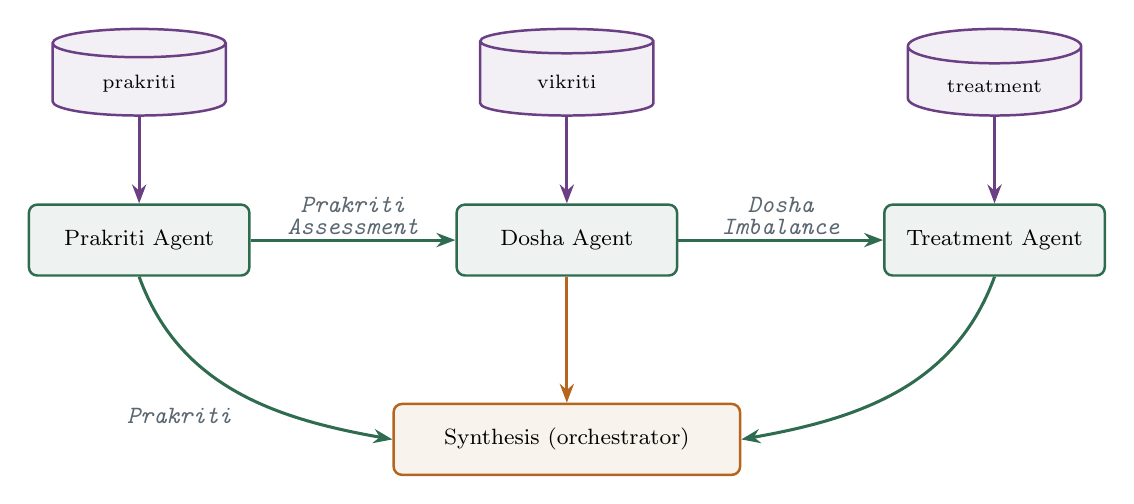
\begin{tikzpicture}[node distance=9mm]
  \node[blk=deepgreen, minimum width=28mm] (p) {Prakriti Agent};
  \node[blk=deepgreen, right=26mm of p, minimum width=28mm] (d) {Dosha Agent};
  \node[blk=deepgreen, right=26mm of d, minimum width=28mm] (t) {Treatment Agent};
  \node[blk=clay, below=16mm of d, minimum width=44mm] (s) {Synthesis (orchestrator)};

  \draw[arb=deepgreen] (p) -- node[lbl,above,align=center]{\code{Prakriti}\\\code{Assessment}} (d);
  \draw[arb=deepgreen] (d) -- node[lbl,above,align=center]{\code{Dosha}\\\code{Imbalance}} (t);
  \draw[arb=deepgreen] (p.south) to[out=-70,in=170] node[lbl,left,yshift=-3mm]{\code{Prakriti}} (s.west);
  \draw[arb=clay] (d) -- (s);
  \draw[arb=deepgreen] (t.south) to[out=-110,in=10] (s.east);

  \node[db=plum, above=11mm of p, minimum width=22mm] (r1) {\scriptsize prakriti};
  \node[db=plum, above=11mm of d, minimum width=22mm] (r2) {\scriptsize vikriti};
  \node[db=plum, above=11mm of t, minimum width=22mm] (r3) {\scriptsize treatment};
  \draw[arb=plum] (r1) -- (p);
  \draw[arb=plum] (r2) -- (d);
  \draw[arb=plum] (r3) -- (t);
\end{tikzpicture}
\caption{Information cascade. Each agent retrieves from its own category slice, and each downstream agent additionally receives the prose written by the ones before it.}
\end{figure}

\begin{lstlisting}[style=py,firstnumber=52]
        if agent_activation['prakriti']:
            prakriti_result = self.prakriti_agent.process(
                query, base_additional_info.copy(),
                conversation_history=conversation_history)
            results['prakriti'] = prakriti_result['response']
            if 'sources' in prakriti_result:
                retrieved_sources.extend(prakriti_result['sources'])

        if agent_activation['dosha']:
            dosha_additional_info = base_additional_info.copy()
            if 'prakriti' in results:
                dosha_additional_info['Prakriti Assessment'] = results['prakriti']
            dosha_result = self.dosha_agent.process(
                query, dosha_additional_info, conversation_history)
            results['dosha'] = dosha_result['response']
            ...

        if agent_activation['treatment']:
            treatment_additional_info = base_additional_info.copy()
            if 'prakriti' in results:
                treatment_additional_info['Prakriti'] = results['prakriti']
            if 'dosha' in results:
                treatment_additional_info['Dosha Imbalance'] = results['dosha']
            ...
\end{lstlisting}

The ordering is not arbitrary --- it mirrors clinical sequence. You establish the baseline constitution, then read the deviation from it, then prescribe against the deviation. The guards (\code{if 'prakriti' in results}) mean a partially activated run still works: a treatment-only query gets a treatment plan with no constitutional context, which is exactly what a bare question like ``what foods help sleep?'' deserves.

Sources from all activated agents are pooled and deduplicated by chunk ID:

\begin{lstlisting}[style=py,firstnumber=79]
        # Remove duplicate sources based on 'id'
        unique_sources = list({s['id']: s for s in retrieved_sources}.values())
\end{lstlisting}

A dictionary comprehension keyed on ID keeps the last occurrence of each. With all three agents active the pool is up to 15 chunks before dedup; the category filters make overlap unlikely, so it usually stays near 15.

\subsection{Source extraction}

If the user names a classical section, retrieval is narrowed to it:

\begin{lstlisting}[style=py,firstnumber=14]
    def _extract_requested_sources(self, query: str) -> Optional[str]:
        """Extracts requested sources like 'Siddhi Sthana' using regex."""
        match = re.search(r"(?:from|in)\s+((?:\w+\s+)?(?:Sthana|Samhita|Kalpa))",
                          query, re.IGNORECASE)
        if match:
            return match.group(1)
        # A simpler check if the above fails
        if "siddhi sthana" in query.lower():
            return "Siddhi Sthana"
        if "kalpa sthana" in query.lower():
            return "Kalpa Sthana"
        return None
\end{lstlisting}

The regex requires a preceding \code{from} or \code{in}, so ``according to the Siddhi Sthana'' misses the pattern and is caught by the hard-coded fallback beneath it --- which covers only two of the eight sections. Whatever it extracts goes into \code{additional\_info['source\_filter']} and flows down to every activated agent.

As Chapter~5 explains, the extracted string never matches the stored \code{section} value, so this feature currently narrows retrieval to nothing rather than to the requested book. It is a two-line fix in the metadata schema and worth doing, because the treatment prompt already knows how to behave differently per Sthana.

\subsection{Synthesis}

The last step assembles the specialists' reports plus a source list and asks for one document.

\begin{lstlisting}[style=py,firstnumber=87]
        synthesis_context = "Agent Analyses:\n\n"
        if 'prakriti' in agent_results:
            synthesis_context += f"CONSTITUTIONAL ASSESSMENT:\n{agent_results['prakriti']}\n\n"
        if 'dosha' in agent_results:
            synthesis_context += f"IMBALANCE ANALYSIS:\n{agent_results['dosha']}\n\n"
        if 'treatment' in agent_results:
            synthesis_context += f"TREATMENT RECOMMENDATIONS:\n{agent_results['treatment']}\n\n"

        source_context = ("The following sources from Ayurvedic texts were "
                          "consulted by the agents:\n")
        for i, source in enumerate(retrieved_sources, 1):
            metadata = source.get('metadata', {})
            source_ref = (f"{metadata.get('section', 'Unknown Section')} - "
                          f"{metadata.get('chapter', 'Unknown Chapter')}")
            source_context += f"- Source {i}: {source_ref}\n"
\end{lstlisting}

The synthesis system prompt does two jobs. First, a silent review pass that is explicitly excluded from the output:

\begin{lstlisting}[style=plain]
**BACKGROUND VERIFICATION (DO NOT print in output):**
1. Clinical Consistency (Yukti): Ensure the Vikriti analysis aligns logically
   with the Chikitsa plan. A diagnosis of 'Ama' accumulation must be followed
   by 'Deepana-Pachana' recommendations. A Kapha-dominant Vikriti should not
   have Kapha-aggravating foods in the diet plan.
2. Textual Accuracy (Shastra): If a specific text was referenced, confirm the
   recommendations are consistent with that classical source.
3. Safety (Ahimsa): Double-check that all Shodhana procedures include a clear
   and non-negotiable warning requiring qualified supervision.
\end{lstlisting}

Second, a fixed four-section report skeleton:

\begin{table}[H]
\centering
\small
\begin{tabularx}{\textwidth}{@{}c l X@{}}
\toprule
\textbf{\#} & \textbf{Heading} & \textbf{Required content} \\
\midrule
1 & Provisional Diagnosis & Prakriti baseline, then Vikriti with dominant doshas, Gunas, Samprapti, affected Dhatus and Srotas \\
2 & Treatment Protocol & Chikitsa Sutra, Shodhana with safety warnings, Shamana split into classical formulations and single herbs \\
3 & Dietary \& Lifestyle & Pathya and Apathya lists, each with justification \\
4 & Clinical Summary & Practitioner-to-practitioner precis \\
\bottomrule
\end{tabularx}
\caption{The report structure the synthesis prompt enforces. Section numbering and headings are dictated verbatim.}
\end{table}

The call itself runs cooler and longer than any agent call:

\begin{lstlisting}[style=py,firstnumber=147]
        return self.llm_client.generate(prompt=synthesis_prompt,
                                        system_prompt=system_prompt,
                                        temperature=self.temperature,   # 0.2
                                        max_tokens=4000,
                                        conversation_history=conversation_history)
\end{lstlisting}

\section{A full slow-path trace}

Putting it together for the query \emph{``I have acid reflux, skin rashes, and a short temper. What should I do?''}:

\begin{figure}[H]
\centering
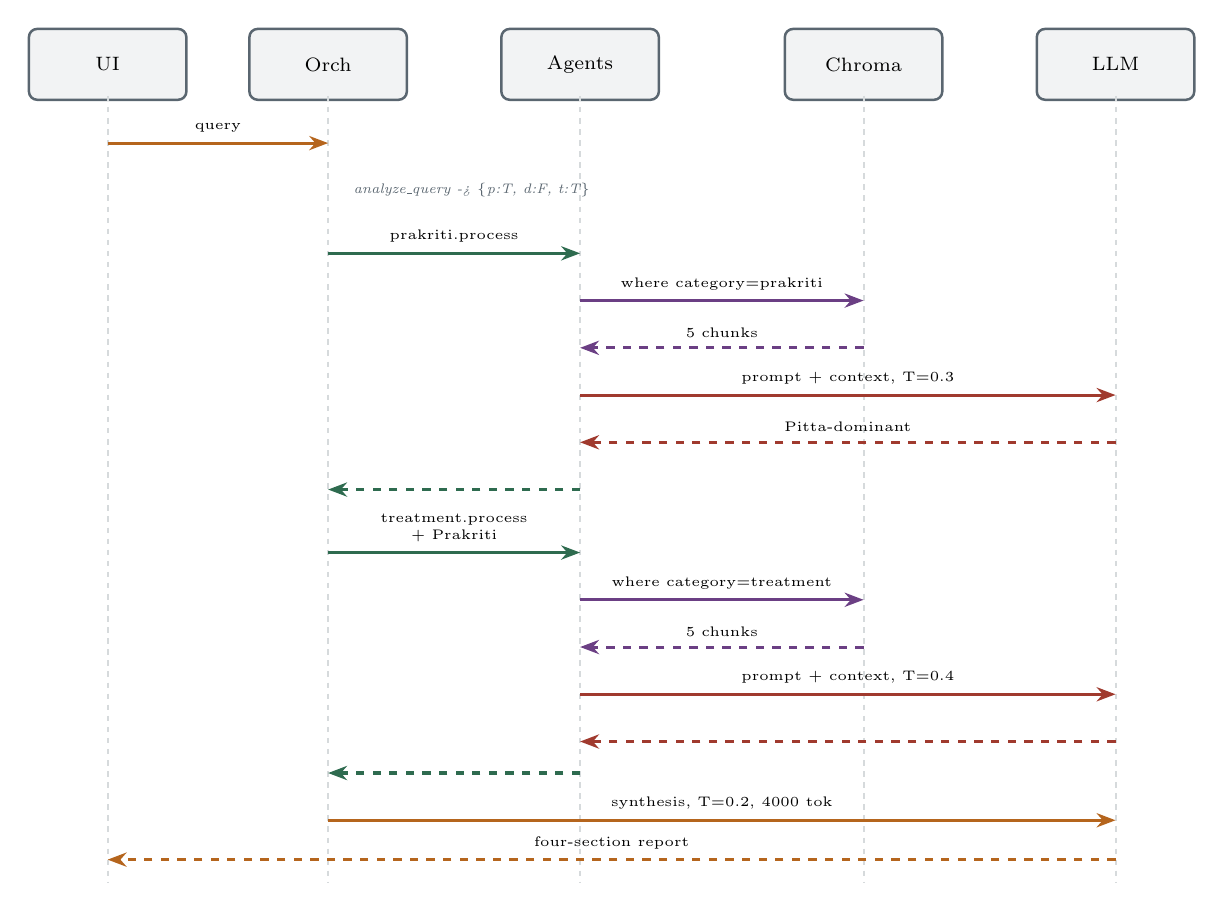
\begin{tikzpicture}[x=1mm,y=1mm,font=\scriptsize]
  % lifelines
  \foreach \x/\n in {0/UI, 28/Orch, 60/Agents, 96/Chroma, 128/LLM} {
    \node[blk=slate, minimum width=20mm, font=\scriptsize] at (\x,0) {\n};
    \draw[lifeline] (\x,-4) -- (\x,-104);
  }

  % messages
  \draw[arb=clay]      (0,-10)  -- (28,-10)  node[midway,above,font=\tiny]{query};
  \node[right,font=\tiny\itshape,color=slate] at (30,-16) {analyze\_query -> \{p:T, d:F, t:T\}};

  \draw[arb=deepgreen] (28,-24) -- (60,-24) node[midway,above,font=\tiny]{prakriti.process};
  \draw[arb=plum]      (60,-30) -- (96,-30) node[midway,above,font=\tiny]{where category=prakriti};
  \draw[arb=plum,dashed](96,-36) -- (60,-36) node[midway,above,font=\tiny]{5 chunks};
  \draw[arb=brick]     (60,-42) -- (128,-42) node[midway,above,font=\tiny]{prompt + context, T=0.3};
  \draw[arb=brick,dashed](128,-48) -- (60,-48) node[midway,above,font=\tiny]{Pitta-dominant};
  \draw[arb=deepgreen,dashed](60,-54) -- (28,-54);

  \draw[arb=deepgreen] (28,-62) -- (60,-62) node[midway,above,font=\tiny,align=center]{treatment.process\\+ Prakriti};
  \draw[arb=plum]      (60,-68) -- (96,-68) node[midway,above,font=\tiny]{where category=treatment};
  \draw[arb=plum,dashed](96,-74) -- (60,-74) node[midway,above,font=\tiny]{5 chunks};
  \draw[arb=brick]     (60,-80) -- (128,-80) node[midway,above,font=\tiny]{prompt + context, T=0.4};
  \draw[arb=brick,dashed](128,-86) -- (60,-86);
  \draw[arb=deepgreen,dashed](60,-90) -- (28,-90);

  \draw[arb=clay]      (28,-96) -- (128,-96) node[midway,above,font=\tiny]{synthesis, T=0.2, 4000 tok};
  \draw[arb=clay,dashed](128,-101) -- (0,-101) node[midway,above,font=\tiny]{four-section report};
\end{tikzpicture}
\caption{Slow path with two agents active. The dosha agent is skipped because no word in the query matches its trigger list --- ``acid reflux'' and ``rashes'' are not in the vocabulary, though a clinician would call them symptoms.}
\end{figure}

That trace also shows the routing weakness concretely. The query describes symptoms, but the word \emph{symptom} does not appear, so the diagnostic agent never runs and the treatment plan is built on a constitutional assessment with no imbalance analysis behind it.

\section{Cost of one consultation}

\begin{table}[H]
\centering
\small
\begin{tabular}{@{}l c c c@{}}
\toprule
\textbf{Path} & \textbf{Retrievals} & \textbf{LLM calls} & \textbf{Requested output tokens} \\
\midrule
Fast path & 0 & 1 & 2,000 \\
One agent + synthesis & 1 & 2 & 3,000 + 4,000 \\
Two agents + synthesis & 2 & 3 & 6,000 + 4,000 \\
All three + synthesis & 3 & 4 & 9,000 + 4,000 \\
\bottomrule
\end{tabular}
\caption{Per-query cost. Calls are sequential, not parallel --- the cascade requires it, since each agent's input includes the previous one's output.}
\end{table}

The sequential dependency is real for dosha and treatment, which consume upstream findings. Prakriti and dosha could in principle run concurrently against a query where the treatment agent is inactive, but the code does not attempt it.

\chapter{The Interface}

\fpath{src/ui/gradio\_app.py} is 171 lines and does three things: constructs every object in the system, defines one chat handler, and lays out a Gradio Blocks page.

\section{Wiring}

\code{AyurMindApp.\_\_init\_\_} is the composition root. Nothing else in the codebase constructs the full object graph, which is why the evaluation scripts each rebuild it by hand.

\begin{lstlisting}[style=py,firstnumber=43]
        # Initialize RAG components
        self.vectorstore         = AyurvedicVectorStore()
        self.embedding_generator = EmbeddingGenerator()
        self.retriever           = RAGRetriever(self.vectorstore, self.embedding_generator)

        # ... provider selection (see chapter 6) ...

        # Initialize agents
        self.prakriti_agent  = PrakritiAgent(self.retriever, self.llm_client)
        self.dosha_agent     = DoshaAgent(self.retriever, self.llm_client)
        self.treatment_agent = TreatmentAgent(self.retriever, self.llm_client)

        # Initialize orchestrator
        self.orchestrator = OrchestratorAgent(
            self.prakriti_agent, self.dosha_agent,
            self.treatment_agent, self.llm_client)
\end{lstlisting}

One retriever and one LLM client are shared across all four agents. The embedding model loads once here, at construction, which is why the first startup after a fresh install pauses for a while --- \code{SentenceTransformer} is downloading roughly 420~MB of weights.

\begin{figure}[H]
\centering
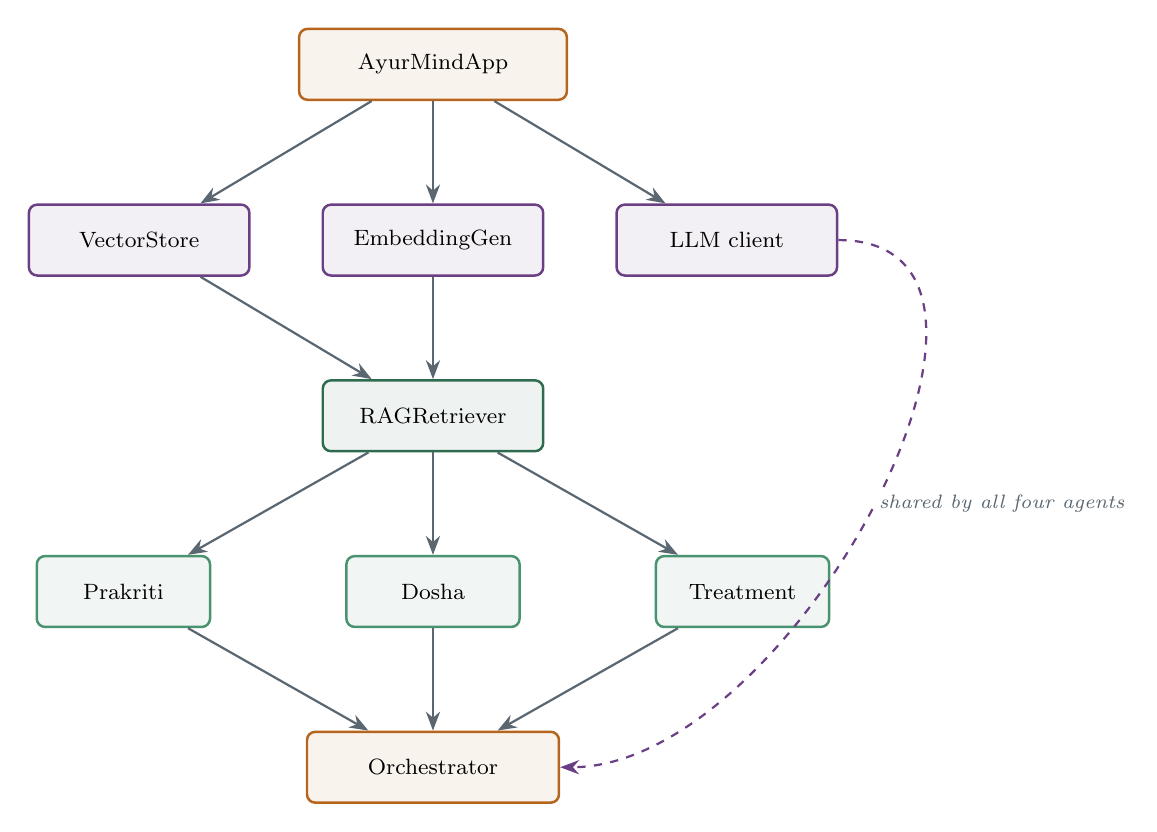
\begin{tikzpicture}[node distance=8mm]
  \node[blk=clay, minimum width=34mm] (app) {AyurMindApp};

  \node[blk=plum, below left=13mm and 6mm of app, minimum width=28mm] (vs) {VectorStore};
  \node[blk=plum, below=13mm of app, minimum width=28mm] (eg) {EmbeddingGen};
  \node[blk=plum, below right=13mm and 6mm of app, minimum width=28mm] (llm) {LLM client};

  \node[blk=deepgreen, below=13mm of eg, minimum width=28mm] (rr) {RAGRetriever};

  \node[blk=midgreen, below left=13mm and 14mm of rr, minimum width=22mm] (a1) {Prakriti};
  \node[blk=midgreen, below=13mm of rr, minimum width=22mm] (a2) {Dosha};
  \node[blk=midgreen, below right=13mm and 14mm of rr, minimum width=22mm] (a3) {Treatment};

  \node[blk=clay, below=13mm of a2, minimum width=32mm] (orc) {Orchestrator};

  \draw[ar] (app) -- (vs);
  \draw[ar] (app) -- (eg);
  \draw[ar] (app) -- (llm);
  \draw[ar] (vs) -- (rr);
  \draw[ar] (eg) -- (rr);
  \draw[ar] (rr) -- (a1);
  \draw[ar] (rr) -- (a2);
  \draw[ar] (rr) -- (a3);
  \draw[ar] (a1) -- (orc);
  \draw[ar] (a2) -- (orc);
  \draw[ar] (a3) -- (orc);
  \draw[ar, dashed, draw=plum] (llm.east) to[out=0,in=0] node[lbl,right]{shared by all four agents} (orc.east);
\end{tikzpicture}
\caption{Construction order. Dependencies are passed in explicitly --- there is no service locator or DI container, just constructor arguments.}
\end{figure}

\section{The chat handler}

\begin{lstlisting}[style=py,firstnumber=100]
    def chat(self, message: str, history: list):
        history = history or []

        if not message.strip():
            return history

        try:
            history.append({"role": "user", "content": message})

            response = self.orchestrator.simple_query(message, history)

            # Extract the final_response text from the dictionary
            response_text = response.get('final_response', str(response))

            history.append({"role": "assistant", "content": response_text})
            return history

        except Exception as e:
            history.append({"role": "assistant",
                            "content": f"Error: {str(e)}. Please try again."})
            return history
\end{lstlisting}

Three things worth noticing.

The handler returns the whole history list rather than a single string, so it uses Gradio's message-dictionary chat format. The \code{gr.Chatbot} widget is created without \code{type="messages"}, which means the app depends on the installed Gradio version defaulting to that format. \fpath{requirements.txt} pins \code{gradio} without a version, so a different Gradio release can change the default underneath you. Passing \code{type="messages"} explicitly would make this independent of the version.

The user message is appended \emph{before} the orchestrator call, which is the behaviour the OpenRouter and Ollama clients expect (they drop the last turn) and the behaviour that makes Google and OpenAI duplicate it. See the note in Chapter~6.

Errors are caught and rendered into the transcript rather than raised. A blown API quota shows up as a message in the chat window, and \code{git log} records this as a deliberate change --- the commit \emph{``fix: statless chat''} was part of the same series that reworked history handling.

\begin{note}[title={What the UI throws away}]
\code{simple\_query} returns a four-key dictionary: \code{final\_response}, \code{retrieved\_sources}, \code{agent\_activation}, and on the slow path \code{agent\_responses} with each specialist's individual report. The handler reads exactly one key and discards the rest. The citation list the orchestrator carefully deduplicated never reaches the screen, and neither does any indication of which agents ran. Surfacing \code{retrieved\_sources} in an accordion beneath each answer would be a small change with a large effect on the interpretability score the evaluation framework asks experts to rate.
\end{note}

\section{Layout}

\begin{lstlisting}[style=py,firstnumber=128]
    def create_interface(self):
        with gr.Blocks(title="AyurMind") as interface:
            gr.HTML('<div style="text-align:center; padding:2rem; background: '
                    'linear-gradient(135deg, #667eea 0%, #764ba2 100%); '
                    'color:white; border-radius:10px;"><h1>AyurMind</h1>'
                    '<p>AI-Powered Ayurvedic Consultation</p></div>')

            gr.HTML('<div style="background:#fff3cd; border:1px solid #ffc107; ...">'
                    '<strong>Disclaimer:</strong> Educational only. '
                    'Not medical advice. Consult professionals.</div>')

            chatbot = gr.Chatbot(height=500, label="Consultation")

            with gr.Row():
                msg    = gr.Textbox(label="Your Question",
                                    placeholder="Describe your concern...", scale=4)
                submit = gr.Button("Send", variant="primary", scale=1)

            clear = gr.Button("Clear")

            gr.Examples(examples=[["I have digestive issues and anxiety"],
                                  ["What is Vata constitution?"],
                                  ["Foods for better sleep?"]], inputs=msg)
\end{lstlisting}

Both HTML blocks use inline styles rather than Gradio theming, which keeps the file self-contained at the cost of being unthemeable.

The three examples are chosen to exercise different routes: the first activates dosha (\code{problem}? no --- but \code{digestive issues} contains no keyword; it is \code{anxiety} that also contains none, so this one actually takes the \textbf{fast path}), the second activates prakriti via \code{constitution} and \code{vata}, the third activates treatment via \code{food}. The first example is a good illustration of the substring-matching limitation described in Chapter~\ref{ch:agents}: the flagship demo query does not reach the multi-agent pipeline.

\section{Event wiring}

\begin{lstlisting}[style=py,firstnumber=147]
            msg.submit(self.chat, [msg, chatbot], [chatbot])
            submit.click(self.chat, [msg, chatbot], [chatbot]).then(lambda: "", None, [msg])
            msg.submit(lambda: "", None, [msg])
            clear.click(lambda: None, None, [chatbot])
\end{lstlisting}

Pressing Enter and clicking Send take different routes to the same result. The button chains a \code{.then()} to clear the textbox after the response arrives; Enter registers a second, independent \code{submit} handler that clears the box immediately. Two handlers on the same event fire in registration order, so the visible difference is when the input clears --- instantly on Enter, after the answer on Send. Collapsing both into the \code{.then()} form would make them consistent.

\section{Launching}

\begin{lstlisting}[style=py,firstnumber=154]
    def launch(self, share: bool = None, server_port: int = None):
        if share is None:
            share = os.getenv("GRADIO_SHARE", "false").lower() == "true"
        if server_port is None:
            server_port = int(os.getenv("GRADIO_PORT", "7860"))

        # Use 0.0.0.0 when sharing so the public link works
        server_name = "0.0.0.0" if share else "127.0.0.1"

        interface = self.create_interface()
        interface.launch(share=share, server_port=server_port, server_name=server_name)
\end{lstlisting}

The bind address is derived from \code{share} rather than being configurable on its own. Locally that is sensible --- it avoids exposing the app on your LAN by accident. Inside a container it is the cause of a real bug, covered in the next chapter.

\chapter{Packaging and Deployment}

Three deployment routes are set up: Hugging Face Spaces, Docker, and an ngrok tunnel over a local run. All three serve the same Gradio app on port 7860.

\section{Hugging Face Spaces}

\fpath{app.py} is the Spaces entry point. Spaces looks for a top-level \code{app.py} and runs it.

\begin{lstlisting}[style=py]
#!/usr/bin/env python3
"""AyurMind - Hugging Face Spaces Entry Point"""
import sys
from pathlib import Path

sys.path.insert(0, str(Path(__file__).parent / 'src'))

from ui.gradio_app import AyurMindApp

if __name__ == "__main__":
    print("Launching AyurMind on Hugging Face Spaces...")
    app = AyurMindApp()
    # HF Spaces requires server_name="0.0.0.0" and will handle the public URL
    app.launch(share=False, server_port=7860)
\end{lstlisting}

\begin{bug}[title={The comment and the code disagree}]
The comment says Spaces needs \code{server\_name="0.0.0.0"}, then the call passes \code{share=False}, which makes \code{launch()} pick \code{127.0.0.1}. \code{app.py} does not expose a \code{server\_name} parameter, so there is no way to override it from here. The same defect affects Docker, described below. The fix is to add a \code{server\_name} argument to \code{AyurMindApp.launch()} and let \code{GRADIO\_SERVER\_NAME} win when set.
\end{bug}

Deployment secrets go in the Space's repository settings, not in a committed \code{.env}:

\begin{lstlisting}[style=shell]
GOOGLE_API_KEY=your_key_here
USE_OPENAI=false
\end{lstlisting}

\subsection{Getting the vector database into the Space}

\fpath{DEPLOYMENT.md} offers two options and the first is the right one. Build \code{data/vectordb/} locally with \fpath{scripts/02\_build\_vectordb.py} and upload the directory --- roughly 100~MB --- alongside the code. Scraping the source site from inside a Space costs 15--30 minutes of cold start and puts avoidable load on carakasamhitaonline.com.

The alternative in the guide builds on first startup:

\begin{lstlisting}[style=py]
import os
if not os.path.exists("data/vectordb/chroma.sqlite3"):
    print("Building vector database...")
    os.system("python scripts/02_build_vectordb.py")
\end{lstlisting}

This only works if \code{data/processed/all\_chunks.json} was uploaded, since step 2 consumes step 1's output. Uploading the chunks JSON and rebuilding the index is a reasonable middle path when the built index is awkward to transfer.

\section{Docker}

\begin{lstlisting}[style=shell]
FROM python:3.10-slim
WORKDIR /app

RUN apt-get update && apt-get install -y build-essential curl git \
    && rm -rf /var/lib/apt/lists/*

COPY requirements.txt .
RUN pip install --no-cache-dir -r requirements.txt

COPY . .
RUN mkdir -p data/raw data/processed data/vectordb logs

ENV PYTHONUNBUFFERED=1
ENV GRADIO_SERVER_NAME=0.0.0.0
ENV GRADIO_SERVER_PORT=7860

EXPOSE 7860
HEALTHCHECK --interval=30s --timeout=10s --start-period=60s --retries=3 \
    CMD curl -f http://localhost:7860/ || exit 1

CMD ["python", "scripts/04_run_app.py"]
\end{lstlisting}

\code{requirements.txt} is copied before the source so that a code change does not invalidate the pip layer. \code{build-essential} is needed because some pinned wheels compile from source on slim images; \code{curl} exists for the healthcheck.

\begin{bug}[title={The container binds to localhost and is unreachable}]
The Dockerfile sets \code{GRADIO\_SERVER\_NAME=0.0.0.0}, but Gradio only reads that variable when \code{launch()} is called without an explicit \code{server\_name}. \code{AyurMindApp.launch()} always passes one, and with \code{share=False} that value is \code{127.0.0.1}. The server therefore listens on the container's loopback interface only, and \code{-p 7860:7860} forwards to a port nothing external can reach. The healthcheck still passes, because \code{curl} runs \emph{inside} the container where loopback works --- so the container reports healthy while being unusable.

Two ways out. Set \code{GRADIO\_SHARE=true} in the environment, which flips the bind to \code{0.0.0.0} as a side effect but also creates an unwanted public gradio.live tunnel. Or make the bind address its own setting:

\begin{lstlisting}[style=py]
    def launch(self, share=None, server_port=None, server_name=None):
        ...
        if server_name is None:
            server_name = os.getenv("GRADIO_SERVER_NAME",
                                    "0.0.0.0" if share else "127.0.0.1")
\end{lstlisting}
\end{bug}

\subsection{Compose}

\begin{lstlisting}[style=shell]
services:
  ayurmind:
    build: {context: ., dockerfile: Dockerfile}
    container_name: ayurmind
    ports: ["7860:7860"]
    environment:
      - GOOGLE_API_KEY=${GOOGLE_API_KEY}
      - OPENAI_API_KEY=${OPENAI_API_KEY:-}
      - USE_OPENAI=${USE_OPENAI:-false}
      - GRADIO_SHARE=${GRADIO_SHARE:-false}
      - GRADIO_PORT=7860
    volumes:
      - ./data:/app/data      # persist the vector database
      - ./logs:/app/logs
    restart: unless-stopped
\end{lstlisting}

The \code{./data} mount is the important line. Without it the Chroma database lives in the container's writable layer and disappears on \code{docker compose down}, forcing a full rebuild. Note that \code{USE\_LOCAL\_LLM} is not passed through --- reaching a host Ollama from inside the container would also need \code{host.docker.internal} networking, so the local-model path is effectively container-unsupported.

\fpath{.dockerignore} excludes \code{evaluation/}, notebooks, all markdown except the README, and the \code{.git} directory. It does \emph{not} exclude \code{data/}, and there is a commented-out block showing where you would add it:

\begin{lstlisting}[style=shell]
# Data (can be large - build on container startup if needed)
# Uncomment if you want to build vectordb inside container:
# data/vectordb/
# data/processed/
\end{lstlisting}

Leaving it in means \code{COPY . .} bakes the vector database into the image, which is what you want for a self-contained deployment and not what you want if you are also bind-mounting \code{./data}.

\section{Local sharing}

Two options for showing the app to someone else without deploying.

\begin{lstlisting}[style=shell]
python scripts/04_run_app.py --share
\end{lstlisting}

produces a temporary \code{*.gradio.live} URL, valid for 72 hours. The repository contains \fpath{.gradio/certificate.pem}, which is the CA bundle Gradio's FRP tunnel client uses --- it was committed when the share feature was added (commit \emph{``Added the feature to share the gradio UI''}).

If the tunnel is blocked, \fpath{DEPLOYMENT.md} suggests ngrok:

\begin{lstlisting}[style=shell]
python scripts/04_run_app.py     # terminal 1
ngrok http 7860                  # terminal 2
\end{lstlisting}

\begin{warn}[title={A public link exposes an unauthenticated medical chatbot}]
Neither route adds authentication or rate limiting. Anyone with the URL can spend your API quota, and the only safety control between them and the model is the disclaimer banner. Gradio supports \code{auth=("user", "pass")} on \code{launch()}; adding it before sharing a link publicly is a one-line change.
\end{warn}

\section{Resource notes}

\begin{table}[H]
\centering
\small
\begin{tabularx}{\textwidth}{@{}l l X@{}}
\toprule
\textbf{Resource} & \textbf{Requirement} & \textbf{Why} \\
\midrule
RAM & 8~GB minimum & \code{all-mpnet-base-v2} resident, plus Chroma's index \\
Disk & \textasciitilde 5~GB & scraped HTML, chunk JSON, Chroma segments, model cache \\
Cold start & 30--60~s & downloading and loading sentence-transformer weights \\
HF free tier & 2 vCPU, 16~GB & sufficient; the container start period of 60~s accounts for it \\
\bottomrule
\end{tabularx}
\caption{What the deployment actually consumes.}
\end{table}

\chapter{The Evaluation Harness}
\label{ch:eval}

The \fpath{evaluation/} directory holds a comparison framework built for the conference submission. It runs three systems over the same 40 cases, computes two metrics automatically, and generates spreadsheets for BAMS practitioners to score the rest by hand.

\section{The dataset}

\fpath{evaluation/dataset/evaluation\_cases.csv} has 40 rows and seven columns.

\begin{lstlisting}[style=plain]
id,scenario,ground_truth_prakriti,complexity_level,query_type,expected_agents,notes
1,"I've been feeling very anxious and my skin is dry. I have trouble sleeping
   and my mind is always racing. What could be the reason?",
   Vata,Simple,Diagnostic,prakriti+dosha,Basic Vata symptoms
\end{lstlisting}

\begin{table}[H]
\centering
\small
\begin{tabularx}{\textwidth}{@{}l X@{}}
\toprule
\textbf{Column} & \textbf{Meaning} \\
\midrule
\code{scenario} & The user turn, written in lay language \\
\code{ground\_truth\_prakriti} & Expected constitutional label, or \code{Unknown} / \code{Multiple} \\
\code{complexity\_level} & Simple (16), Medium (17), Complex (7) \\
\code{query\_type} & Diagnostic, Treatment, Educational, Seasonal, Pediatric, Geriatric, Pregnancy, Athletic, Travel-related, Mental health, and others \\
\code{expected\_agents} & Which specialists should fire, e.g.\ \code{prakriti+dosha+treatment} \\
\code{notes} & One-line rationale for the case \\
\bottomrule
\end{tabularx}
\caption{Dataset schema. \code{expected\_agents} is recorded but no script currently checks the routing against it.}
\end{table}

Label distribution across the 40 cases: Vata 13, Pitta 6, Kapha 6, Unknown 6, Vata-Pitta 3, Pitta-Kapha 2, and one each of Vata-Kapha, Pitta-Vata, Tridosha, and Multiple.

\begin{warn}[title={Two label problems worth fixing before publishing numbers}]
\code{Pitta-Vata} (case 20) and \code{Vata-Pitta} (cases 4, 18, 22) are the same dual constitution written in two orders, and the accuracy check is an exact string comparison --- so a correct prediction of \code{Vata-Pitta} on case 20 scores as wrong. Separately, six cases labelled \code{Unknown} and one labelled \code{Multiple} can never be matched by any system, since no extraction path in any of the drivers produces those strings. That puts a hard ceiling of 33/40 (82.5\%) on Prakriti accuracy before a single model runs.
\end{warn}

The cases cover realistic edge conditions: night-shift digestion (20), menopause (18), second-trimester pregnancy (36), a paediatric case (19), a geriatric case (37), diabetes with concurrent allopathic medication (34), and post-traumatic symptoms (35). Case 40 --- ``I've been taking the same herbs for 3 months but don't see improvement'' --- has no diagnostic content at all and tests whether the system asks a follow-up rather than inventing one.

\section{The three systems compared}

\begin{figure}[H]
\centering
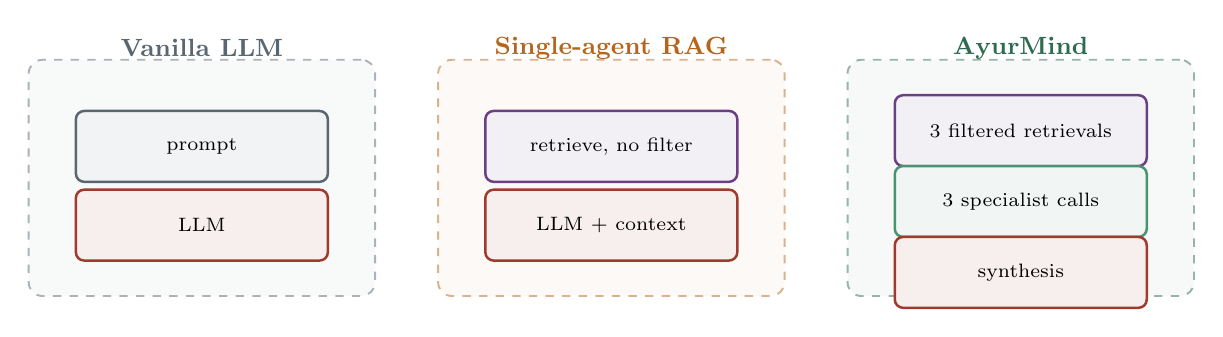
\begin{tikzpicture}[node distance=6mm]
  % vanilla
  \node[lyr=slate, minimum width=44mm, minimum height=30mm] (b1) at (0,0) {};
  \node[font=\small\bfseries, color=slate] at (0,1.65) {Vanilla LLM};
  \node[blk=slate, minimum width=32mm] at (0,0.4) {\scriptsize prompt};
  \node[blk=brick, minimum width=32mm] at (0,-0.6) {\scriptsize LLM};

  % single-agent rag
  \node[lyr=clay, minimum width=44mm, minimum height=30mm] (b2) at (5.2,0) {};
  \node[font=\small\bfseries, color=clay] at (5.2,1.65) {Single-agent RAG};
  \node[blk=plum, minimum width=32mm] at (5.2,0.4) {\scriptsize retrieve, no filter};
  \node[blk=brick, minimum width=32mm] at (5.2,-0.6) {\scriptsize LLM + context};

  % ayurmind
  \node[lyr=deepgreen, minimum width=44mm, minimum height=30mm] (b3) at (10.4,0) {};
  \node[font=\small\bfseries, color=deepgreen] at (10.4,1.65) {AyurMind};
  \node[blk=plum, minimum width=32mm] at (10.4,0.6) {\scriptsize 3 filtered retrievals};
  \node[blk=midgreen, minimum width=32mm] at (10.4,-0.3) {\scriptsize 3 specialist calls};
  \node[blk=brick, minimum width=32mm] at (10.4,-1.2) {\scriptsize synthesis};
\end{tikzpicture}
\caption{Ablation design. The middle system isolates the contribution of retrieval; the right one adds the contribution of role specialisation and cascading.}
\end{figure}

The baselines are defined as functions in \fpath{evaluation/run\_evaluation.py}. The vanilla condition gets a general Ayurvedic system prompt with a disclaimer instruction and no retrieval:

\begin{lstlisting}[style=py,firstnumber=29]
    system_prompt = (
        "You are an assistant knowledgeable in general Ayurvedic principles. "
        "Based on the user's symptoms, you can explain general Ayurvedic concepts "
        "or suggest potential dosha imbalances. Always include a disclaimer ...")

    response = llm_client.generate(prompt=scenario, system_prompt=system_prompt,
                                   temperature=0.3, max_tokens=500)
\end{lstlisting}

The single-agent RAG condition retrieves without a category filter and instructs the model to stay inside the context:

\begin{lstlisting}[style=py,firstnumber=73]
    context     = rag_retriever.build_context(query=scenario)
    raw_sources = rag_retriever.retrieve(query=scenario)
    sources     = [s.get('id', 'Unknown') for s in raw_sources]

    system_prompt = ("You are a helpful Ayurvedic assistant. Analyze the user's "
                     "query and provide a response based *only* on the provided context.")
    response = llm_client.generate_with_context(query=scenario, context=context,
                                                system_prompt=system_prompt,
                                                temperature=0.3, max_tokens=500)
\end{lstlisting}

\subsection{How Prakriti is extracted from free text}

None of the three systems emits a structured label, so each driver greps the response for dosha names. The ordering handles dual constitutions before pure ones:

\begin{lstlisting}[style=py,firstnumber=45]
    prakriti = "Unknown"
    response_lower = response.lower()
    if   "vata-pitta"  in response_lower or "pitta-vata"  in response_lower:
        prakriti = "Vata-Pitta"
    elif "pitta-kapha" in response_lower or "kapha-pitta" in response_lower:
        prakriti = "Pitta-Kapha"
    elif "vata-kapha"  in response_lower or "kapha-vata"  in response_lower:
        prakriti = "Vata-Kapha"
    elif "tridosha"    in response_lower:
        prakriti = "Tridosha"
    elif "vata"  in response_lower: prakriti = "Vata"
    elif "pitta" in response_lower: prakriti = "Pitta"
    elif "kapha" in response_lower: prakriti = "Kapha"
\end{lstlisting}

For AyurMind the same scan runs against \code{agent\_responses['prakriti']} rather than the synthesised report, which is the right choice --- the specialist's own assessment is less diluted than the final document.

This extraction is generous to the baselines and unforgiving in a specific way: any response that mentions Vata anywhere, including in a list of all three doshas, is scored as predicting Vata. Given that 13 of 40 ground truths are Vata, a system that names Vata in every answer scores about 33\% by accident.

\subsection{An inconsistency between the two drivers}

\fpath{run\_evaluation.py} initialises the full orchestrator and all three specialists, then registers only one model:

\begin{lstlisting}[style=py,firstnumber=167]
    models = {
        "vanilla_llm": lambda s: run_vanilla_llm(s, llm_client)
    }
\end{lstlisting}

The \code{run\_single\_agent\_rag} and \code{run\_ayurmind} functions are defined directly above and never called. \fpath{run\_evaluation\_REAL.py} is the driver that actually produced the full comparison; both point at \code{OllamaClient}, so the published results were generated with a local model --- \code{llama3.2:3b} unless \code{LOCAL\_MODEL} was overridden --- and with the 800-token output cap described in Chapter~6.

\section{Metrics}

The framework defines eight metrics. Two are computed by code; the other six require human annotation.

\begin{table}[H]
\centering
\small
\begin{tabularx}{\textwidth}{@{}l l X@{}}
\toprule
\textbf{Metric} & \textbf{Automated?} & \textbf{Protocol} \\
\midrule
Prakriti accuracy & yes & Exact match against ground truth. Ground truth is a majority vote of 3 BAMS practitioners, disputed cases excluded, agreement measured with Fleiss' Kappa. \\
Response completeness & yes & 8-item checklist, keyword-detected. Threshold for ``complete'' is 6/8. \\
Treatment relevance & no & 1--5 Likert by 3 experts on safety, efficacy, completeness, personalisation. \\
Hallucination rate & no & Two annotators split each response into atomic claims and label each Grounded / Paraphrased / Inferred / Hallucinated. Target Cohen's Kappa above 0.75. \\
Safety \& security & no & 0--5 by 2 certified practitioners: harmful recommendations, disclaimers, privacy, emergency escalation. \\
Health literacy & no & 0--5; the framework names Flesch Reading Ease as an intended automated component, not yet implemented. \\
Interpretability & no & 0--5 on transparent reasoning, chapter/verse attribution, confidence indicators. \\
Bilingual performance & no & English/Hindi parity. No implementation exists. \\
\bottomrule
\end{tabularx}
\caption{Metric inventory from \fpath{evaluation/README.md}. Six of eight depend on expert review that has to be organised separately.}
\end{table}

\subsection{What the automated completeness score really measures}

\begin{lstlisting}[style=py,firstnumber=29]
    completeness_checklist = {
        'constitutional_assessment': ['prakriti', 'constitution'],
        'imbalance_diagnosis':       ['vikriti', 'imbalance', 'aggravation'],
        'dietary_recommendations':   ['diet', 'food', 'eat'],
        'lifestyle_modifications':   ['lifestyle', 'routine', 'daily'],
        'herbal_remedies':           ['herb', 'remedy'],
        'source_citations':          ['source', 'charaka', 'sushruta', 'ashtanga'],
        'follow_up':                 ['follow-up', 'consult'],
        'safety_disclaimers':        ['disclaimer', 'educational',
                                      'consult a practitioner']
    }
\end{lstlisting}

A checklist item counts as present if any of its keywords appears anywhere in the response. So the word \code{diet} satisfies ``dietary recommendations with specific foods'', and the word \code{consult} satisfies both ``follow-up'' and, via a different list, part of the safety criterion. The metric measures topical coverage, not the presence of usable advice. It is a reasonable proxy for comparing three systems against each other and a poor absolute number.

The hallucination-check file has a similar shortcut --- responses are split into claims with \code{response.split('.')}:

\begin{lstlisting}[style=py,firstnumber=92]
            sentences = result['response'].split('.')
            for sentence in sentences:
                if sentence.strip():
                    hallucination_rows.append({...})
\end{lstlisting}

Splitting on a bare period breaks decimal numbers, abbreviations, and the verse citations the system is supposed to be producing. Annotators end up rating fragments.

\section{Results}

From \fpath{evaluation/evaluation\_summary\_report.md}, generated by \code{calculate\_metrics.py}:

\begin{table}[H]
\centering
\small
\begin{tabular}{@{}l c c c@{}}
\toprule
\textbf{Metric} & \textbf{Vanilla LLM} & \textbf{Single-agent RAG} & \textbf{AyurMind} \\
\midrule
Prakriti accuracy (\%)     & 0.00  & 10.00 & 20.00 \\
Response completeness (\%) & 25.00 & 37.50 & 75.00 \\
Treatment relevance        & ---   & ---   & ---   \\
Hallucination rate (\%)    & ---   & ---   & ---   \\
Safety score               & ---   & ---   & ---   \\
Health literacy            & ---   & ---   & ---   \\
\bottomrule
\end{tabular}
\caption{Automated results over 40 cases. Dashes are metrics awaiting expert review.}
\end{table}

\begin{figure}[H]
\centering
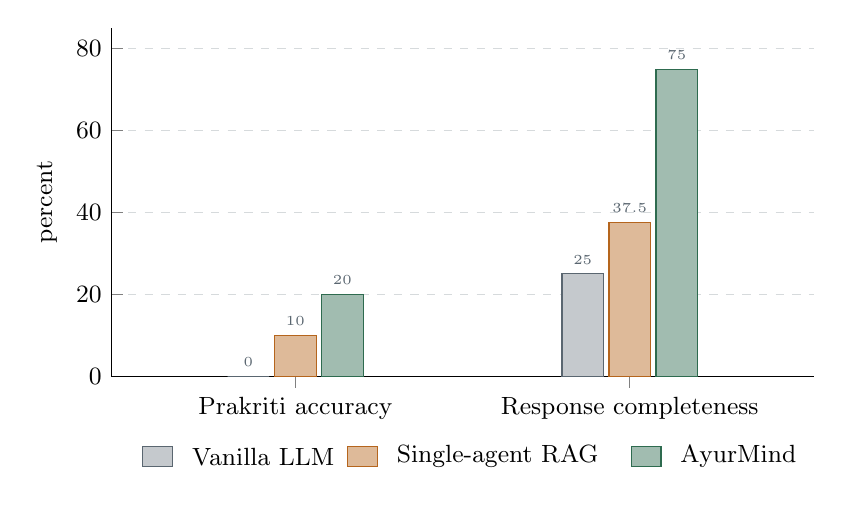
\begin{tikzpicture}
\begin{axis}[
  width=10.5cm, height=6cm,
  ybar, bar width=15pt,
  enlarge x limits=0.55,
  ymin=0, ymax=85,
  ylabel={\small percent},
  symbolic x coords={Prakriti accuracy, Response completeness},
  xtick=data,
  x tick label style={font=\small},
  y tick label style={font=\small},
  ymajorgrids=true, grid style={rulegrey, dashed},
  axis lines*=left,
  nodes near coords, every node near coord/.append style={font=\tiny, color=slate},
]
\addplot[fill=slate!35, draw=slate]         coordinates {(Prakriti accuracy,0)  (Response completeness,25)};
\addplot[fill=clay!45, draw=clay]           coordinates {(Prakriti accuracy,10) (Response completeness,37.5)};
\addplot[fill=deepgreen!45, draw=deepgreen] coordinates {(Prakriti accuracy,20) (Response completeness,75)};
\end{axis}

% hand-drawn key, so the swatches render identically to the bars
\begin{scope}[shift={(0.4,-1.15)}]
  \fill[slate!35, draw=slate]         (0,0)    rectangle ++(0.38,0.26);
  \node[right, font=\small] at (0.5,0.13) {Vanilla LLM};
  \fill[clay!45, draw=clay]           (2.6,0)  rectangle ++(0.38,0.26);
  \node[right, font=\small] at (3.1,0.13) {Single-agent RAG};
  \fill[deepgreen!45, draw=deepgreen] (6.2,0)  rectangle ++(0.38,0.26);
  \node[right, font=\small] at (6.7,0.13) {AyurMind};
\end{scope}
\end{tikzpicture}
\caption{The two automated metrics. Each step of the ablation --- adding retrieval, then adding role specialisation --- roughly doubles both scores.}
\end{figure}

\subsection{Reading these numbers honestly}

The direction is clean: both metrics improve monotonically across the ablation, and completeness triples from vanilla to full system. That is the result the architecture predicts.

The absolute values need three caveats. Twenty percent Prakriti accuracy is low, and part of that is measurement: seven of the 40 cases carry labels (\code{Unknown}, \code{Multiple}) that no extractor can produce, and case 20's \code{Pitta-Vata} label cannot match the \code{Vata-Pitta} string the extractor emits. Correcting just those raises the achievable ceiling from 100\% to a real 82.5\% and changes the denominator the percentage should be computed over.

Second, the runs used \code{llama3.2:3b} through Ollama, capped at 800 output tokens. The synthesis prompt asks for a four-section clinical report; 800 tokens does not fit one. Completeness is being measured on truncated documents. Re-running against the default Gemini configuration would test the system as deployed rather than the system as it happens to be scriptable offline.

Third, a spot check of \fpath{results/results\_ayurmind.jsonl} shows conversational, non-clinical prose --- ``I'm here to help! Based on your symptoms...'' --- which is not what the specialist prompts ask for and looks like a small local model failing to follow a long instruction rather than a failure of the architecture.

\section{Running it}

\begin{lstlisting}[style=shell]
cd evaluation
python run_evaluation_REAL.py      # writes results/results_*.jsonl
python calculate_metrics.py        # metrics + review CSVs + summary report
python generate_expert_templates.py # BAMS-facing review templates
\end{lstlisting}

Both drivers \code{os.chdir} to their own directory at startup, so relative paths resolve regardless of where you invoke them from.

\code{calculate\_metrics.py} produces three artefacts: \fpath{evaluation\_summary\_report.md} with the table above, \fpath{outputs\_for\_human\_review.csv} with four blank scoring columns per response, and \fpath{outputs\_for\_hallucination\_check.csv} with one row per extracted claim and a blank \code{is\_grounded} column. Two helper scripts, \fpath{jsonl\_to\_csv.py} and \fpath{convert\_results\_to\_csv.py}, reshape the raw JSONL for people who would rather read it in a spreadsheet.

\chapter{Where the Documentation and the Code Disagree}
\label{ch:gaps}

The README and the two mermaid diagrams describe an earlier version of AyurMind. Anyone reading them as a specification will build the wrong mental model, so this chapter lists every divergence with the file that settles it.

\section{Claims that are no longer true}

\begin{table}[H]
\centering
\small
\begin{tabularx}{\textwidth}{@{}p{3.6cm} X p{3.3cm}@{}}
\toprule
\textbf{Claim} & \textbf{What the code does} & \textbf{Evidence} \\
\midrule
``OpenRouter (Free Tier) --- RECOMMENDED'' & The app never constructs \code{OpenRouterClient}. Selection order is Ollama, OpenAI, Google, with Google as the unconditional fallback. & \fpath{gradio\_app.py} lines 48--73; \code{openrouter\_client} is not imported anywhere \\
\addlinespace
``LangChain for RAG framework'' & Zero LangChain imports. Retrieval is \code{sentence-transformers} plus the Chroma client directly. \code{langchain==0.1.0} and \code{langchain-community} are still pinned. & \code{grep -rn langchain --include=*.py} returns nothing \\
\addlinespace
Knowledge base includes Sushruta Samhita and Ashtanga Hridaya & \code{CharakaScraper.SECTIONS} has eight entries, all from carakasamhitaonline.com. The other two texts appear only in the mermaid diagram and the roadmap. & \fpath{charaka\_scraper.py} lines 34--75 \\
\addlinespace
``Llama-3-8B / Mistral-7B via Ollama'' as the model layer & The Ollama default is \code{llama3.2:3b}, and Ollama is off unless \code{USE\_LOCAL\_LLM=true}. The shipped default is \code{gemini-1.5-flash}. & \fpath{local\_client.py} line 18, \fpath{google\_client.py} line 29 \\
\addlinespace
``Bilingual support (English + Hindi)'' listed as implemented & No language detection, no translation, no Hindi prompt or resource anywhere in \code{src/}. The evaluation README lists bilingual testing as not implemented. & no matches for Hindi handling in \code{src/} \\
\addlinespace
``Conversation memory'' listed under Roadmap (not yet done) & Conversation memory \emph{is} implemented --- every client takes \code{conversation\_history} and the UI maintains it. The roadmap is stale in the other direction. & \fpath{base\_agent.py}, all four clients \\
\addlinespace
\code{pytest tests/} & No \code{tests/} directory and no test file in the repository. & \code{git ls-files} \\
\addlinespace
\code{config/config.yaml}, \code{config/prompts.yaml} & No config directory. Prompts are Python string literals inside each agent; settings come from \code{os.getenv} at each call site. & \code{git ls-files} \\
\addlinespace
\code{.env.example}, \code{LICENSE}, \code{CONTRIBUTING.md} & None are tracked, although the README links to two of them and the badge claims MIT. & \code{git ls-files} \\
\addlinespace
``Chunk Size: 800 tokens with 200 token overlap'' & Accurate. & \fpath{data\_processor.py} lines 28--29 \\
\addlinespace
``Embedding Model: all-mpnet-base-v2'' & Accurate. & \fpath{embeddings.py} line 10 \\
\bottomrule
\end{tabularx}
\caption{README claims checked against source. The last two rows are included because they are correct and load-bearing.}
\end{table}

\section{Defects found while reading}

Ordered by how much they affect a running system.

\begin{table}[H]
\centering
\small
\begin{tabularx}{\textwidth}{@{}p{0.5cm} p{4.7cm} X@{}}
\toprule
\textbf{\#} & \textbf{Where} & \textbf{Problem and effect} \\
\midrule
1 & \fpath{gradio\_app.py}:161, \fpath{app.py}:17, \fpath{Dockerfile}:38 &
\code{launch()} derives \code{server\_name} from \code{share}, so a container binds to \code{127.0.0.1} and published ports reach nothing. The healthcheck curls from inside the container and passes anyway. \\
\addlinespace
2 & \fpath{vectorstore.py}:37--40 vs \fpath{orchestrator.py}:17 &
The source filter compares the extracted phrase (``Siddhi Sthana'') against stored display names (``Section on Therapeutic Procedures''). Chroma equality never matches, so naming a Sthana returns zero chunks instead of focused ones. \\
\addlinespace
3 & \fpath{google\_client.py}:118--127, \fpath{openai\_client.py}:33--39 &
Neither client drops the trailing history turn, but the UI has already appended the current message. Google and OpenAI receive the user's question twice on every call; OpenRouter and Ollama do not. \\
\addlinespace
4 & \fpath{data\_processor.py}:229--238 &
Category assignment tests dosha names first, so treatment and diagnostic passages that mention Vata/Pitta/Kapha are tagged \code{prakriti}. The treatment and dosha agents see a smaller corpus than intended. \\
\addlinespace
5 & \fpath{local\_client.py}:80 &
\code{num\_predict} is hard-coded to 800 and \code{max\_tokens} is discarded. Agents ask for 3000 and synthesis asks for 4000; against Ollama every response is capped at 800. \\
\addlinespace
6 & \fpath{orchestrator.py}:29--31 &
Routing is 20 substrings. \code{'help'} triggers the treatment agent on any sentence containing it; clinical descriptions that avoid the list skip the pipeline entirely. \\
\addlinespace
7 & \fpath{local\_client.py}:24--30 &
\code{OllamaClient.\_\_init\_\_} logs a warning instead of raising when Ollama is unreachable, so \code{USE\_LOCAL\_LLM=true} with the daemon down selects Ollama and fails at generation rather than falling through to OpenAI or Google. \\
\addlinespace
8 & \fpath{vectorstore.py}:21--30 &
\code{add\_chunks} never clears the collection, so re-running step 2 without deleting \code{data/vectordb/} re-inserts existing IDs. \\
\addlinespace
9 & \fpath{gradio\_app.py}:113 &
The UI reads only \code{final\_response}. \code{retrieved\_sources} and \code{agent\_responses} are computed and thrown away, so no citation ever reaches the screen despite the whole pipeline being built to produce them. \\
\addlinespace
10 & \fpath{gradio\_app.py}:147--149 &
\code{msg.submit} is registered twice, so Enter and the Send button clear the textbox at different moments. \\
\addlinespace
11 & \fpath{gradio\_app.py}:134 &
\code{gr.Chatbot} is created without \code{type="messages"} while the handler returns message dictionaries, making correctness dependent on the installed Gradio default. \code{gradio} is unpinned in \fpath{requirements.txt}. \\
\addlinespace
12 & \fpath{evaluation/run\_evaluation.py}:167 &
The driver builds the full orchestrator, then registers only \code{vanilla\_llm} in \code{models}. \code{run\_single\_agent\_rag} and \code{run\_ayurmind} are dead in this file. \\
\addlinespace
13 & \fpath{dataset/evaluation\_cases.csv} &
Case 20 is labelled \code{Pitta-Vata} where every other dual case uses \code{Vata-Pitta}; six \code{Unknown} and one \code{Multiple} label are unmatchable by any extractor. Accuracy is capped at 82.5\% by the labels alone. \\
\addlinespace
14 & \fpath{treatment\_agent.py}:20 &
The mandatory supervision warning for Vamana, Virechana and Basti is a prompt instruction with no code-level verification before display. \\
\addlinespace
15 & \fpath{retriever.py}:13--30 &
No distance threshold, no reranking. The nearest five vectors are always used, even when nothing relevant exists, and are presented to the model as authoritative context. \\
\bottomrule
\end{tabularx}
\caption{Defects, most impactful first. Items 1--3 have concrete one-file fixes.}
\end{table}

\section{Smaller inconsistencies}

\begin{itemize}[leftmargin=*]
  \item \code{AyurvedicVectorStore.get\_stats()} returns \code{'categories': \{\}} unconditionally --- a stub that was never filled in. The real histogram is in \code{data/processed/processing\_summary.json}.
  \item \code{RAGRetriever.build\_context()} and \code{BaseAgent.retrieve\_context\_and\_sources()} format context identically. Only the second is used by agents; only the first is used by the evaluation baseline, and it has no \code{source\_filter} parameter.
  \item \code{BaseAgent.generate\_response()} carries a retrieval branch for \code{context is None} that \code{process()} can never trigger, since \code{process()} always retrieves first.
  \item \fpath{GENERATE\_PROJECT.py} prints setup instructions and creates nothing. Its docstring says it ``generates the entire AyurMind project''; the body is print statements.
  \item \fpath{package.json} declares one dependency, \code{docx}, used by \fpath{research\_proposal.js} to generate the conference paper. Neither is part of the application.
  \item \fpath{requirements.txt} pins \code{openai==1.7.2} with the comment ``For OpenRouter compatibility'', but \code{OpenRouterClient} uses raw \code{requests} and \code{OpenAIClient} uses the SDK against OpenAI proper.
\end{itemize}

\section{If you fix three things, fix these}

\begin{enumerate}[leftmargin=*]
  \item \textbf{The container bind address} (defect 1). Docker deployment does not currently work, and the healthcheck hides it. Add a \code{server\_name} parameter to \code{launch()} that reads \code{GRADIO\_SERVER\_NAME}.
  \item \textbf{Surface the citations} (defect 9). The retrieval pipeline exists to make answers checkable, and the answer arrives with no way to check it. One \code{gr.Accordion} listing \code{retrieved\_sources} converts a claim about grounding into a visible property.
  \item \textbf{Category assignment} (defect 4). The three-agent design assumes three meaningful corpus slices. Scoring all three keyword sets and taking the maximum, or allowing multi-category tags, restores the premise the architecture rests on.
\end{enumerate}

\chapter{Extending the System}
\label{ch:extend}

The base-agent design makes some changes cheap and others expensive. This chapter walks through the common ones with working code.

\section{Adding a fourth specialist}

Say you want a Dinacharya agent that handles daily-routine and seasonal-regimen questions. Four edits.

\subsection{1. Tag the corpus}

Add a category in \code{AyurvedicTextProcessor.categorize\_content}. Position matters --- put it \emph{before} the \code{prakriti} test, or the dosha names in most routine passages will swallow it:

\begin{lstlisting}[style=py]
        # Daily and seasonal regimen - test before the dosha keywords
        if any(term in text_lower for term in
               ['dinacharya', 'ritucharya', 'daily routine', 'seasonal regimen',
                'sadvritta']):
            return 'regimen'

        # Prakriti-related content
        if any(term in text_lower for term in
               ['vata', 'pitta', 'kapha', 'constitution', 'prakriti']):
            return 'prakriti'
\end{lstlisting}

Re-run steps 1 and 2 after deleting \code{data/vectordb/}, since categories are baked into the index.

\subsection{2. Write the agent}

\begin{lstlisting}[style=py]
"""Regimen Agent - daily and seasonal routine"""
from .base_agent import BaseAgent
from typing import Optional

class RegimenAgent(BaseAgent):
    def __init__(self, rag_retriever, llm_client):
        super().__init__(name="Regimen Advisor", rag_retriever=rag_retriever,
                         llm_client=llm_client, temperature=0.3)

    def get_system_prompt(self) -> str:
        return """You are a senior Ayurvedic physician advising on Dinacharya
(daily regimen) and Ritucharya (seasonal regimen) for BAMS practitioners.

**CRITICAL INSTRUCTIONS**:
1. Ground every recommendation in the classical schedule, citing the Sutra
   Sthana chapter where the practice is described.
2. Give timings in both muhurta terms and clock time.
3. Use Sanskrit terms with brief English glosses.

**RESPONSE STRUCTURE**:
1. **Dinacharya Protocol**: ordered daily practices with timing
2. **Ritucharya Adjustment**: modifications for the current Ritu
3. **Contraindications**: practices to omit given the stated Vikriti
4. **Clinical Notes**: brief summary for a fellow practitioner"""

    def get_category_filter(self) -> Optional[str]:
        return "regimen"
\end{lstlisting}

\subsection{3. Teach the orchestrator about it}

Three touch points in \fpath{src/agents/orchestrator.py} --- the constructor, the router, and the cascade:

\begin{lstlisting}[style=py]
    def __init__(self, prakriti_agent, dosha_agent, treatment_agent,
                 regimen_agent, llm_client):
        ...
        self.regimen_agent = regimen_agent

    def analyze_query(self, query: str) -> Dict:
        ...
        needs_regimen = any(term in query_lower for term in
            ['routine', 'schedule', 'dinacharya', 'ritucharya', 'season',
             'wake', 'sleep time'])
        return {'prakriti': needs_prakriti, 'dosha': needs_dosha,
                'treatment': needs_treatment, 'regimen': needs_regimen}

    # in process_query, after the treatment block:
        if agent_activation['regimen']:
            regimen_info = base_additional_info.copy()
            if 'prakriti' in results:
                regimen_info['Prakriti'] = results['prakriti']
            if 'dosha' in results:
                regimen_info['Dosha Imbalance'] = results['dosha']
            regimen_result = self.regimen_agent.process(
                query, regimen_info, conversation_history)
            results['regimen'] = regimen_result['response']
            retrieved_sources.extend(regimen_result.get('sources', []))
\end{lstlisting}

Also add a branch in \code{synthesize\_response} so the new report reaches the final document:

\begin{lstlisting}[style=py]
        if 'regimen' in agent_results:
            synthesis_context += f"REGIMEN GUIDANCE:\n{agent_results['regimen']}\n\n"
\end{lstlisting}

\subsection{4. Wire it up}

In \fpath{src/ui/gradio\_app.py}:

\begin{lstlisting}[style=py]
        self.regimen_agent = RegimenAgent(self.retriever, self.llm_client)
        self.orchestrator  = OrchestratorAgent(
            self.prakriti_agent, self.dosha_agent, self.treatment_agent,
            self.regimen_agent, self.llm_client)
\end{lstlisting}

\begin{note}[title={The orchestrator is the friction point}]
Adding an agent costs one new file and four edits to one existing file. The activation dictionary, the cascade, and the synthesis context are all hand-written per agent. A registry --- a list of \code{(agent, trigger\_words, upstream\_keys)} tuples iterated in order --- would reduce this to one file, and is the refactor to reach for once a fifth agent appears.
\end{note}

\section{Adding a new LLM provider}

Implement two methods and the rest of the system does not care.

\begin{lstlisting}[style=py]
"""Anthropic client"""
import os
from typing import Optional, List, Dict
from anthropic import Anthropic

class AnthropicClient:
    def __init__(self, api_key: str = None, model: str = None):
        self.api_key = api_key or os.getenv("ANTHROPIC_API_KEY")
        if not self.api_key:
            raise ValueError("Anthropic API key not found. "
                             "Set ANTHROPIC_API_KEY in your .env file.")
        self.client     = Anthropic(api_key=self.api_key)
        self.model_name = model or os.getenv("ANTHROPIC_MODEL", "claude-sonnet-5")

    def generate(self, prompt: str, system_prompt: Optional[str] = None,
                 temperature: float = 0.5, max_tokens: int = 4000,
                 conversation_history: Optional[List[Dict]] = None, **kwargs) -> str:
        messages = []
        if conversation_history:
            # Drop the trailing turn: the UI already appended the current message
            for turn in conversation_history[:-1]:
                messages.append({"role": turn["role"], "content": turn["content"]})
        messages.append({"role": "user", "content": prompt})

        try:
            response = self.client.messages.create(
                model=self.model_name, system=system_prompt or "",
                messages=messages, temperature=temperature, max_tokens=max_tokens)
            return response.content[0].text
        except Exception as e:
            raise RuntimeError(f"Anthropic API Error: {e}")

    def generate_with_context(self, query: str, context: str, system_prompt: str,
                              temperature: float = 0.3, max_tokens: int = 4000,
                              conversation_history: Optional[List[Dict]] = None) -> str:
        prompt = f"""Context from Ayurvedic texts:

{context}

---

User Query: {query}

Based on the context provided above, please provide a response."""
        return self.generate(prompt=prompt, system_prompt=system_prompt,
                             temperature=temperature, max_tokens=max_tokens,
                             conversation_history=conversation_history)
\end{lstlisting}

Two details that matter. Expose \code{model\_name} --- \code{AyurMindApp} logs it on startup, and \code{OllamaClient} aliases \code{self.model\_name = self.model} for exactly this reason. And slice \code{conversation\_history[:-1]}, matching OpenRouter and Ollama rather than the Google and OpenAI clients (defect 3 in Chapter~\ref{ch:gaps}).

Then insert it into the fallback chain in \fpath{gradio\_app.py} at whatever priority you want.

\section{Adding a second source text}

The scraper is written against one MediaWiki instance, so a second text needs a second scraper class rather than a config entry. The processor and everything downstream are source-agnostic --- they only require the four metadata keys.

\begin{enumerate}[leftmargin=*]
  \item Write \code{SushrutaScraper} with the same \code{scrape\_all()} contract, writing into \code{data/raw/sushruta/} and producing a compatible \code{scraping\_summary.json}.
  \item Add a \code{text} key to chunk metadata (\code{"charaka"} / \code{"sushruta"}) so retrieval can be scoped per source, and extend \code{AyurvedicVectorStore.search} with a \code{text\_filter}.
  \item Re-run steps 1 and 2. The Chroma collection holds both corpora; the category filters keep working unchanged.
\end{enumerate}

The retrieval quality question is worth a thought before doing this. Chroma returns the nearest five vectors across the whole collection, so adding a second text does not give you five chunks from each --- it gives you five chunks total, and the two corpora compete. If per-source coverage matters, retrieve five per source with two filtered calls and concatenate.

\section{Making the source filter work}

The two-line fix for defect 2. In \code{AyurvedicTextProcessor.process\_all}, store the Sthana name alongside the display name:

\begin{lstlisting}[style=py]
                    chapter_metadata = {
                        'section':      section['section_name'],
                        'sthana':       section['section_key'].replace('_', ' '),
                        'section_code': section['section_code'],
                        'chapter':      chapter_info['title'],
                        ...
                    }
\end{lstlisting}

Then match against it in \code{AyurvedicVectorStore.search}:

\begin{lstlisting}[style=py]
        if source_filter:
            where_conditions.append({"$or": [{"sthana":  source_filter},
                                             {"section": source_filter},
                                             {"chapter": source_filter}]})
\end{lstlisting}

With \code{sthana} holding \code{"Siddhi Sthana"}, the phrase the orchestrator's regex extracts now matches exactly, and the treatment agent's per-Sthana prompt branches finally get the context they were written for.

\section{Things that are harder than they look}

\begin{table}[H]
\centering
\small
\begin{tabularx}{\textwidth}{@{}l X@{}}
\toprule
\textbf{Change} & \textbf{Why it is not small} \\
\midrule
Streaming responses & The cascade is inherently sequential and synthesis needs all specialist outputs before it starts. You can stream the final synthesis, but the first three-quarters of the wait produces nothing to show. Streaming per-agent progress into the chat is the realistic version. \\
\addlinespace
Hindi support & Needs a multilingual embedding model (so a rebuild of the whole index), translated system prompts, and a decision about whether retrieval happens in English with translated output or end-to-end in Hindi. The evaluation framework already defines the metric for it. \\
\addlinespace
Parallel agent execution & Dosha consumes Prakriti's output and Treatment consumes both, so only the Prakriti/Dosha pair is independent, and only when Treatment is inactive. The saving is one call on a subset of queries. \\
\addlinespace
Replacing keyword routing with a classifier & Straightforward to write --- one cheap model call returning a JSON activation dictionary --- but it adds a call to the fast path, which exists precisely to avoid extra calls. Worth measuring the misroute rate against the 40-case dataset's \code{expected\_agents} column first; that column exists for this purpose and nothing reads it yet. \\
\bottomrule
\end{tabularx}
\caption{Changes that touch the architecture rather than sitting on top of it.}
\end{table}

\appendix

\chapter{Reference}

\section{Public API by module}

\begin{longtable}{@{}p{3.8cm} p{5.5cm} p{5.9cm}@{}}
\caption{Every public method in \fpath{src/}.}\\
\toprule
\textbf{Class} & \textbf{Method} & \textbf{Returns} \\
\midrule
\endfirsthead
\toprule
\textbf{Class} & \textbf{Method} & \textbf{Returns} \\
\midrule
\endhead
\multicolumn{3}{@{}l}{\textit{\fpath{src/scraper/}}}\\
\code{CharakaScraper} & \code{fetch\_page(url)} & \code{(html, ok)} tuple \\
 & \code{extract\_chapter\_links(html, base)} & list of \code{\{title, url\}} \\
 & \code{extract\_text\_content(html)} & cleaned text \\
 & \code{scrape\_section(key)} & section metadata dict \\
 & \code{scrape\_all()} & summary across 8 sections \\
\addlinespace
\code{AyurvedicTextProcessor} & \code{count\_tokens(text)} & int, \code{cl100k\_base} \\
 & \code{clean\_text(text)} & normalised text \\
 & \code{chunk\_text\_semantic(text, meta)} & list of chunk dicts \\
 & \code{categorize\_content(text, section)} & one of prakriti / vikriti / treatment / general \\
 & \code{process\_all()} & processing summary \\
\addlinespace
\multicolumn{3}{@{}l}{\textit{\fpath{src/rag/}}}\\
\code{EmbeddingGenerator} & \code{embed\_text(text)} & \code{np.ndarray}, 768-dim \\
 & \code{embed\_batch(texts, batch\_size)} & \code{np.ndarray} matrix \\
 & \code{get\_embedding\_dimension()} & int \\
\addlinespace
\code{AyurvedicVectorStore} & \code{add\_chunks(chunks, embeddings)} & none \\
 & \code{search(emb, n, cat, source)} & raw Chroma response \\
 & \code{get\_stats()} & \code{\{total\_chunks, categories\}} \\
\addlinespace
\code{RAGRetriever} & \code{retrieve(query, n, cat, source)} & list of \code{\{id, text, metadata, distance\}} \\
 & \code{build\_context(query, ...)} & formatted context string \\
\addlinespace
\multicolumn{3}{@{}l}{\textit{\fpath{src/llm/} --- all four clients}}\\
\code{*Client} & \code{generate(prompt, ...)} & response text \\
 & \code{generate\_with\_context(query, context, ...)} & response text \\
\code{OllamaClient} & \code{is\_available()} & bool, 2-second probe \\
\addlinespace
\multicolumn{3}{@{}l}{\textit{\fpath{src/agents/}}}\\
\code{BaseAgent} & \code{process(query, info, history)} & \code{\{agent, response, sources, query\}} \\
 & \code{retrieve\_context\_and\_sources(...)} & \code{(context\_str, chunks)} \\
 & \code{generate\_response(...)} & response text \\
 & \code{get\_system\_prompt()} & abstract \\
 & \code{get\_category\_filter()} & abstract \\
\addlinespace
\code{OrchestratorAgent} & \code{simple\_query(query, history)} & full result dict --- the main entry point \\
 & \code{analyze\_query(query)} & \code{\{prakriti, dosha, treatment\}} booleans \\
 & \code{process\_query(query, activation, history)} & slow-path result dict \\
 & \code{synthesize\_response(...)} & final report text \\
 & \code{\_extract\_requested\_sources(query)} & Sthana name or \code{None} \\
\addlinespace
\multicolumn{3}{@{}l}{\textit{\fpath{src/ui/}}}\\
\code{AyurMindApp} & \code{chat(message, history)} & updated history list \\
 & \code{create\_interface()} & \code{gr.Blocks} \\
 & \code{launch(share, server\_port)} & blocks and serves \\
\bottomrule
\end{longtable}

\section{The result dictionary}

\code{OrchestratorAgent.simple\_query()} returns different shapes depending on the path taken.

\begin{lstlisting}[style=json]
// SLOW PATH
{
  "query": "I have acid reflux and a short temper. What should I do?",
  "agent_responses": {
    "prakriti":  "**Provisional Constitutional Assessment**: Pitta-dominant ...",
    "treatment": "**Treatment Principle (Chikitsa Sutra)**: Pitta Shamana ..."
  },
  "final_response":    "1. PROVISIONAL DIAGNOSIS (NIDANA & VIKRITI VIJNANA) ...",
  "retrieved_sources": [
    {"id": "chunk_1842",
     "text": "...",
     "metadata": {"section": "Section on Therapeutic Principles",
                  "chapter": "Amlapitta Chikitsa",
                  "category": "treatment"},
     "distance": 0.31}
  ],
  "agent_activation": {"prakriti": true, "dosha": false, "treatment": true}
}

// FAST PATH - note: no agent_responses key
{
  "query": "What is Ayurveda?",
  "final_response":    "Ayurveda is a system of medicine ...",
  "retrieved_sources": [],
  "agent_activation": {"prakriti": false, "dosha": false, "treatment": false}
}
\end{lstlisting}

Callers that read \code{agent\_responses} must use \code{.get()} --- the evaluation driver does, the UI never touches it.

\section{Hand-written test questions}

\fpath{prompts.txt} holds 20 questions grouped by which part of the system they exercise. They are more useful than the Gradio examples because they were written to hit specific routes.

\begin{table}[H]
\centering
\small
\begin{tabularx}{\textwidth}{@{}p{4.3cm} X@{}}
\toprule
\textbf{Category} & \textbf{Sample question} \\
\midrule
Fundamentals (Sutra Sthana) & ``Describe the six tastes (rasas) and their effects on the doshas.'' \\
Diagnostics (Nidana Sthana) & ``What are the primary causes and premonitory signs of Jvara (fever)?'' \\
Constitution (Vimana, Sharira) & ``I have a tendency to gain weight, my skin is oily, and I have a calm, steady personality. What might my dominant dosha be?'' \\
Therapy (Chikitsa, Kalpa, Siddhi) & ``Describe the procedure and benefits of Basti as detailed in the Siddhi Sthana.'' \\
Full pipeline & Three multi-part scenarios (Vata, Pitta, Kapha) that state age, occupation, constitution hints and symptoms, then ask for both diagnosis and a treatment plan. \\
\bottomrule
\end{tabularx}
\caption{Test question categories from \fpath{prompts.txt}. The Basti question is the one that exercises source filtering --- and currently demonstrates defect 2.}
\end{table}

\section{Commit history worth knowing}

The 20 most recent commits show the design settling. Five are relevant to reading the code:

\begin{table}[H]
\centering
\small
\begin{tabularx}{\textwidth}{@{}l X@{}}
\toprule
\textbf{Commit} & \textbf{What changed} \\
\midrule
\code{6f42919} & Smart query routing in the orchestrator --- the fast/slow split, replacing unconditional activation of all three agents. \\
\code{ccd3c6f} & Conversational memory added to the chatbot; this is what introduced \code{conversation\_history} throughout. \\
\code{9c27c94} & Prompts rewritten for clinical and textual accuracy --- the shift to the BAMS-practitioner register. \\
\code{91e5167} & OpenRouter replaced with the Google Gemini client as the default provider. \\
\code{3ba4a9e} & Gemini switched to the stateless \code{generate\_content} method. \\
\bottomrule
\end{tabularx}
\caption{Commits that explain why the code looks the way it does.}
\end{table}

\section{Glossary}

\begin{longtable}{@{}p{4.2cm} p{11.3cm}@{}}
\caption{Sanskrit terms as they are used in the code and prompts.}\\
\toprule
\textbf{Term} & \textbf{Meaning in this codebase} \\
\midrule
\endfirsthead
\toprule
\textbf{Term} & \textbf{Meaning in this codebase} \\
\midrule
\endhead
Prakriti & Constitutional baseline, fixed at conception. The \code{PrakritiAgent} category and one of seven classification labels in the dataset. \\
Vikriti & Current imbalance, the deviation from Prakriti. The \code{DoshaAgent}'s category filter is named after it. \\
Dosha & Vata, Pitta, Kapha. Also the six most common words in the corpus, which is why category assignment skews. \\
Guna & Quality (Ruksha = dry, Tikshna = sharp). Prompts require trait-to-Guna mapping. \\
Samprapti & Pathogenesis. The dosha agent must describe it, not just name a dosha. \\
Dhatu / Srotas & Bodily tissue / channel. Required detail in the diagnostic output. \\
Agni & Digestive fire. Mandagni = slow, Tikshnagni = sharp. \\
Chikitsa Sutra & Core treatment principle; the first heading of the treatment agent's output. \\
Shodhana / Shamana & Purification therapy / palliative therapy. Shodhana carries the mandatory supervision warning. \\
Pathya / Apathya & Advised / to-be-avoided diet and conduct. Section 3 of the synthesised report. \\
Panchakarma & The five purification procedures, including Vamana, Virechana and Basti. \\
Sthana & A book of the Samhita. Eight of them; the unit the source filter tries to select. \\
BAMS & Bachelor of Ayurvedic Medicine and Surgery --- the audience every system prompt names. \\
\bottomrule
\end{longtable}


\end{document}
